\documentclass[11pt]{article}
\usepackage{amsthm}
\newenvironment{sol}[1][]{\par\noindent\textbf{Solution #1}\ }{\qed\par}

% \usepackage{amsmath,amssymb,amsthm,amsfonts,bm}
% \usepackage{geometry}
% \usepackage{hyperref}
% \usepackage{mathtools}
% \usepackage{enumitem}
% \usepackage{authblk}
\newtheorem{property}{Property}
\usepackage{graphicx}
\usepackage{subcaption}
\usepackage{float}
%__________________________________
%————|Pacakages|———————————————————
%----------------------------------
\usepackage[utf8]{inputenc}
\usepackage[T1]{fontenc}
\usepackage{amsmath,amssymb,amsthm,mathtools}
\usepackage{mathrsfs,bm,color}
\usepackage{fancyhdr,lastpage}
\usepackage[shortlabels]{enumitem}
\usepackage{calc}
\usepackage{bbm}
\usepackage{graphicx}
\usepackage{upgreek}
\usepackage{lmodern}
\usepackage[normalem]{ulem}
\usepackage{verbatim}
\usepackage{bbm}
%\usepackage{ntheorem}
\usepackage{stmaryrd}
\usepackage{amsmath}
% \usepackage{amstex}
\usepackage{amssymb}
\usepackage{dsfont}
\usepackage{amsthm}
\usepackage{hyperref}
\hypersetup{
	colorlinks,
	linkcolor={red!50!black},
	citecolor={red!80!black},
	urlcolor={blue!80!black}
}
\usepackage[numbers]{natbib}
\usepackage{xcolor}

\usepackage{graphicx}

\usepackage{amsfonts}%
\usepackage{dsfont}

%--------------------------------
\def\ra{{\rightarrow}}
\newcommand{\Var}{\operatorname{Var}}


\parindent=1em
\allowdisplaybreaks
\usepackage[hmargin=2cm,vmargin=2cm]{geometry}


%--Enumerate----


%___________________________________
%—|Eqs,Theorems,Lemma,Proofs, etc|——
%-----------------------------------

\numberwithin{equation}{section}

\usepackage{thmtools}
\declaretheorem[thmbox=M,name=Theorem,numberwithin=section]{theo}
\declaretheorem[name=Proposition,thmbox=M,numberwithin=section]{prop}
\declaretheorem[name=Lemma,thmbox=S,numberwithin=section]{lem}
%\declaretheorem[name=Definition,thmbox=M,numberlike=theorem]{defn}
\declaretheorem[name=Corollary,thmbox=M,numberwithin=section]{cor}
\declaretheorem[name=Conjecture,thmbox=M,numberwithin=section]{con}
\declaretheorem[name=Hypothesis,thmbox=S,numberwithin=section]{hyp}
\theoremstyle{definition}
\newtheorem{exam}{Example}[section]
\newtheorem{defn}{Definition}[section]
\newtheorem{rem}{Remark}[section]
\newtheorem{exo}{Exercise}[section]
\newtheorem{ass}{Assumption}[section]
\theoremstyle{plain}

\makeatletter
\renewenvironment{proof}[1][\proofname]{\par
	\pushQED{\qed}%
	\normalfont \topsep6\p@\@plus6\p@\relax
	\trivlist
	\item[\hskip\labelsep
	\sffamily\bfseries
	#1\@addpunct{.}]\ignorespaces
}{%
	\popQED\endtrivlist\@endpefalse
}
\makeatother


%__________________________________
%————|Commands/defs|———————————————
%----------------------------------

%--font--------------------
\newcommand{\jump}{{\vskip 0.3cm \noindent }}


%--english math mode-------
\newcommand{\for}{\mbox{ for }}
\newcommand{\with}{\mbox{ with }}
\renewcommand{\and}{\mbox{ and }}

%--usual functions---------
\newcommand{\e}{\mathrm{e}}

%--Field/usual sets--------
\newcommand{\N}{\mathbb{N}}
\newcommand{\Z}{\mathbb{Z}}
\newcommand{\Q}{\mathbb{Q}}
\newcommand{\R}{\mathbb{R}}
\newcommand{\C}{\mathbb{C}}
\renewcommand{\H}{\mathbb{H}}

\newcommand{\D}{\mathbb{D}}
\newcommand{\T}{\mathbb{T}}
\newcommand{\B}{\mathbb{B}}
\renewcommand{\S}{\mathbb{S}}
\newcommand{\Sn}{\mathbb{S}^{N-1}}

%--Analysis----------------
\newcommand{\dd}{\mathrm d}
\newcommand{\I}{\mathbb{I}}
%\newcommand{\Ind}[1]{\ensuremath{ \I_{\{#1\}}}}
\newcommand{\Ind}[1]{\1_{(#1)}}

%--Ortho. Pol--------------
\newcommand{\polclass}[1]{\ensuremath{\mathrm{#1}}}
\newcommand{\He}{\polclass{He}}
\newcommand{\Hek}{\polclass{He}_k}
\newcommand{\La}{\polclass{La}}
\newcommand{\Lak}{\polclass{La}_k}
\newcommand{\Ja}{\polclass{Ja}}
\newcommand{\Jak}{\polclass{Ja}_k}
\newcommand{\op}{\polclass{P}}
\newcommand{\opk}{\polclass{P}_k}


%--Proba-------------------
\newcommand{\E}{\mathbb{E}}
\renewcommand{\P}{\mathbb{P}}
\def\as{{ \mathrm{a.s.}  }}
\def\ed{\stackrel{{\mathcal{D}}}{=}}
\def\iid{\stackrel{{\mathrm{i.i.d}}}{\sim}}

%--Lin. Algebra------------

    %usual set-------
    \newcommand{\setsqrmat}[1]{\ensuremath{
     \mathrm{M}_{#1}(\R)
    }}
    \newcommand{\setsymmat}[1]{\ensuremath{
     \mathrm{M}^{(\mathrm{sym})}_{#1}(\R)
    }}
   
    
\newcommand{\<}{\ensuremath{ \langle }}
\renewcommand{\>}{\ensuremath{ \rangle }}
\newcommand{\vect}[1]{\ensuremath{\boldsymbol{\mathbf{#1}}}}
\newcommand{\rdmvect}[1]{\ensuremath{\bm{#1}}}
\newcommand{\mat}[1]{\ensuremath{\boldsymbol{\mathbf{#1}}}}
\newcommand{\rdmmat}[1]{\ensuremath{\bm{#1}}}
\newcommand{\tens}[1]{ {\ensuremath{\underline{\boldsymbol{\mathbf{#1}}}}}}
\newcommand{\rdmtens}[1]{ {\ensuremath{\underline{\bm{#1}}}}}
\newcommand{\diag}[1]{\ensuremath{\mat{D}_{\vect{#1}} }}
\newcommand{\Tr}{\ensuremath{\mathrm{Tr}}}
\renewcommand{\det}{\ensuremath{\mathrm{det}}}
\newcommand{\rank}{\ensuremath{\mathrm{rank}}}
%•Norms
\newcommand{\norm}[1]{\ensuremath{ \|#1 \|}}
\newcommand{\normop}[1]{\ensuremath{ \|#1 \|_{\mathrm{op}} }} 

%\newcommand{\norm2}[1]{\ensuremath{ \|#1 \|_{2} }}
\newcommand{\normp}[1]{\ensuremath{ \|#1 \|_{p} }}
\newcommand{\normf}[1]{\ensuremath{ \|#1 \|_{\mathrm{F}} }}
\newcommand{\scalar}[1]{\ensuremath{ \< #1 \>}}

%--classical ensembles of RMT--
%•Gaussian ensembles
\newcommand{\classens}[1]{\ensuremath{\mathsf{#1}}}
\newcommand{\GE}{\ensuremath{{ \classens{GU_{\beta}E}}}}
\newcommand{\GOE}{\ensuremath{{ \classens{GOE}}}}
\newcommand{\GUE}{\ensuremath{{ \classens{GUE}}}}
\newcommand{\GSE}{\ensuremath{{ \classens{GSE}}}}
%•Laguerre ensembles
\newcommand{\LE}{\ensuremath{{ \classens{LU_{\beta}E}}}}
\newcommand{\LOE}{\ensuremath{{ \classens{LOE}}}}
\newcommand{\LUE}{\ensuremath{{ \classens{LUE}}}}
\newcommand{\LSE}{\ensuremath{{ \classens{LSE}}}}
%•Laguerre ensembles
\newcommand{\JE}{\ensuremath{{ \classens{JU_{\beta}E}}}}
\newcommand{\JOE}{\ensuremath{{ \classens{JOE}}}}
\newcommand{\JUE}{\ensuremath{{ \classens{JUE}}}}
\newcommand{\JSE}{\ensuremath{{ \classens{JSE}}}}
%•Circular ensembles
\newcommand{\CE}{\ensuremath{{ \classens{CU_{\beta}E}}}}
\newcommand{\COE}{\ensuremath{{ \classens{COE}}}}
\newcommand{\CUE}{\ensuremath{{ \classens{CUE}}}}
\newcommand{\CSE}{\ensuremath{{ \classens{CSE}}}}
%•Haar Groups
\newcommand{\grpUNb}{\ensuremath{\classens{U}_{\beta}(N)}}
\newcommand{\grpUN}{\ensuremath{ \classens{U}(N)}}
\newcommand{\grpON}{\ensuremath{ \classens{O}(N)}}
\newcommand{\grpSpN}{\ensuremath{ \classens{Sp}(N)}}

%--free proba-------------------------
\newcommand{\rectbox}{{\mathpalette\scaledboxplus\relax}}
\newcommand{\scaledboxplus}[2]{\scalebox{2}[0.95]{$#1\normalboxplus$}}
\newcommand{\recplus}{\fboxsep0pt\fbox{\rule{0.5em}{0pt}\rule{0pt}{0.5ex}}}

%--Partitions/permutations-----------
\newcommand{\classpartition}[1]{\ensuremath{\vect{#1}}}
\newcommand{\classpartitionset}[1]{\ensuremath{\mathcal{}{#1}}}
\newcommand{\partlambda}{\ensuremath{ \classpartition{\uplambda} }}
\newcommand{\partmu}{\ensuremath{ \classpartition{\upmu} }}
\newcommand{\partnu}{\ensuremath{ \classpartition{\upnu} }}
\newcommand{\partpi}{\ensuremath{ \classpartition{\uppi} }}

\newcommand{\partofint}[1]{\ensuremath{ \classpartitionset{P}{#1}}}
\newcommand{\partofk}{\ensuremath{ \classpartitionset{P}(k)}}
\newcommand{\nonpartofint}[1]{\ensuremath{ \classpartitionset{NC}(#1)}}
\newcommand{\nonpartofk}{\ensuremath{ \classpartitionset{NC}(k)}}
\newcommand{\sumpovern}{\ensuremath{\sum_{\partlambda \vdash n }}}
\newcommand{\sumpoverk}{\ensuremath{\sum_{\partlambda \vdash k }}}

\newcommand{\classpermutation}[1]{\ensuremath{#1}}
\newcommand{\permsigma}{\ensuremath{ \classpermutation{\upsigma} }}
\newcommand{\permtau}{\ensuremath{\classpermutation{\uptau}}}

%--symm. polynomials------------------
\newcommand{\classsympol}[1]{\ensuremath{\mathrm{#1}}}

\newcommand{\jack}{\classsympol{J}}
\newcommand{\jackpl}{\classsympol{J}_{\partlambda}}
\newcommand{\jackplb}{\classsympol{J}_{\partlambda}^{(\beta/2)}}
\newcommand{\jackpmu}{\classsympol{J}_{\partmu}}
\newcommand{\jackpmub}{\classsympol{J}_{\partmu}^{(\beta/2)}}
\newcommand{\jackpnu}{\classsympol{J}_{\partnu}}
\newcommand{\jackpnub}{\classsympol{J}_{\partnu}^{(\beta/2)}}

\newcommand{\schur}{\classsympol{s}}
\newcommand{\schurpl}{\classsympol{s}_{\partlambda}}
\newcommand{\schurpmu}{\classsympol{s}_{\partmu}}
\newcommand{\schurpnu}{\classsympol{s}_{\partnu}}
\newcommand{\LRcoeff}{c_{\partlambda,\partmu}^{\partnu}}
\newcommand{\JLRcoeff}{c_{\partlambda,\partmu}^{\partnu}(\beta/2)}


%--article-specific------------
\def\LocLip{{\mathrm{Lip_{loc}}  }}
\def\ks{{k_{\star}}}
\def\Yf{{ \rdmmat{Y}^{(f)}  }}

\def\coeffk{{\vartheta_k(f)}}
\def\coeffks{{\vartheta_{\ks}(f)}}
\def\varfZ{{\vartheta_0(f^2) - \vartheta_0(f)^2 }}
\def\coeffkn{{\vartheta_k(f_t)}}

\def\xk{{\vect{x}^k}}
\def\xks{{\vect{x}^\ks}}
\newcommand{\pert}{\mathrm{pert}}
\def\fm{{f_M}}
\def\fn{{f_t}}
\def\fdm{{f_{\delta,M}}}
\def\fdmp{{f_{\delta,M}^{\pert}}}
\def\fnp{{f_{t}^{\pert}}}
\def\fdmpt{{\Tilde{f}_{\delta,M}^{\pert} }}
\def\fnpt{{\Tilde{f}_{t}^{\pert} }}
%\def\Ytf{{  \rdmmat{\tilde Y}^{(f_L)}  }}
\def\Ytf{{\rdmmat{Y}_{L}^{(f_L)} }}
\def\Ytfdm{{ \rdmmat{\tilde Y}^{(\fdm)}  }}
\def\Ytfdmp{{ \rdmmat{\tilde Y}^{(\fdmp)}  }}
%\def\Ytfnp{{ \rdmmat{\tilde Y}^{(\fnp)}  }}
\def\Ytfnp{{\rdmmat{Y}_{L}^{(\fnp)} }}
\def\Ytfdmpt{{ \rdmmat{\tilde Y}^{(\fdmpt)}  }}
\def\Yfm{{ \rdmmat{Y}^{(\fm)}  }}
\def\Yfdm{{ \rdmmat{Y}^{(\fdm)}  }}
\def\Yfdmp{{ \rdmmat{Y}^{(\fdmp)}  }}
\def\Yfdmpt{{ \rdmmat{Y}^{(\fdmpt)}  }}

\def\wkZ{{w^{(k)}_Z}}
\def\tC{\widetilde{\mat C}}
\def\tY{\widetilde{\rdmmat Y}}

\def\coeffkfdm{{\vartheta_k(\fdm)}}
\def\coeffksfdm{{\vartheta_{\ks}(\fdm)}}
\def\coeffkfdmp{{\vartheta_k(\fdmp)}}
\def\coeffksfdmp{{\vartheta_{\ks}(\fdmp)}}
\def\coeffkfnp{{\vartheta_k(\fnp)}}
\def\coeffksfnp{{\vartheta_{\ks}(\fnp)}}

\def\Lpdx{{L^p(\dd x)}}
\def\Ltwodx{{L^2(\dd x)}}
\def\Lfourdx{{L^4(\dd x)}}

\def\LpZ{{L^p(\mu_Z)}}
\def\LoneZ{{L^1(\mu_Z)}}
\def\LtwoZ{{L^2(\mu_Z)}}
\def\LfourZ{{L^4(\mu_Z)}}
\def\LinfZ{{L^{\infty}(\mu_Z)}}

%--commands crafted for two channels mode--
\newcommand{\bkt}[2]{B^{({#1}), t}_{#2}}
\newcommand{\tbt}[1]{\vect{b}^{t}_{#1}}
\newcommand{\bttt}[0]{\tilde{\vect{b}}^{t}}
\newcommand{\akt}[2]{A^{({#1}), t}_{#2}}
\newcommand{\tat}[1]{\mat{A}^{t}_{#1}}
\newcommand{\ts}[2]{\mat{S}_{#1, #2}}
\newcommand{\trn}[2]{\mat{R}_{#1, #2}}
\newcommand{\tsig}[2]{\mat{\Sigma}^{#1}_{#2}}
\newcommand{\xat}[3]{\hat{x}^{({#1}), #2}_{#3}}
\newcommand{\xtt}[2]{\vect{x}^{#1}_{#2}}
\newcommand{\xttt}[1]{\tilde{\vect{x}}^{#1}}


\def\tib{\vect{b}}
\def\tia{\mat{A}}
\def\tix{\vect{x}}
\def\xone{x^{(1)}}
\def\xtwo{x^{(2)}}
\def\oner{\tilde{1}_R}
\def\onel{\tilde{1}_L}
\def\ovN{{\frac{1}{N}}}
\def\ovsN{{\frac{1}{\sqrt{N}}}}
\def\dovN{{\frac{\mat{\Delta}^{-1}}{N}}}
\def\calij{\mathcal{I}-\mathcal{J}}
\def\calijs{\mathcal{I}-\mathcal{J^*}}
\def\kerij{\mathrm{Ker}(\mathcal{I}-\mathcal{J})}
\def\kerijs{\mathrm{Ker}(\mathcal{I}-\mathcal{J}^*)}

%--commands crafted for tensor mode--
\newcommand{\Tind}[2]{T_{#1 ... #2}}

%--maths symbol commands--
\newcommand\normvert[1]{\left\lVert{#1}\right\rVert}
\newcommand{\para}[1]{\left( {#1} \right)}
\newcommand{\brac}[1]{\left[ {#1} \right]}


%--other commands-----


\newcommand\given[1][]{\:#1\vert\:}
\DeclareMathOperator{\1}{\mathbbm{1}}

\newcommand{\ba}{{\beta}}
\newcommand{\bb}{{\beta_{SNR}}}
\newcommand{\bc}{{\beta_{S}}}
\newcommand{\cR}{\mathcal{R}}
\newcommand{\cL}{\mathcal{L}}
\newcommand{\cG}{\mathcal{G}}
\newcommand{\cB}{\mathcal{B}}
\newcommand{\cS}{\mathcal{S}}
\newcommand{\cH}{\mathcal{H}}
\newcommand{\sD}{\mathscr{D}}
\newcommand{\sO}{\mathcal{O}}
\newcommand{\so}{\mathcal{o}}
\newcommand{\cQ}{\mathcal{Q}}
\newcommand{\sS}{\mathscr{S}}
\newcommand{\sE}{\mathscr{E}}
\newcommand{\sM}{\mathcal{M}}
\newcommand{\sP}{\mathscr{P}}
\newcommand{\cM}{\mathcal{M}}
\newcommand{\sC}{\mathscr{C}}
\newcommand{\cC}{\mathcal{C}}
\newcommand{\sI}{\mathscr{S}}
\newcommand{\sL}{\mathscr{L}}
\newcommand{\sX}{\mathcal{X}}
\newcommand{\cI}{{\mathcal I}}
\newcommand{\bpi}{\bm{\pi}}

\newcommand{\ncal}{\mathcal{N}}
\renewcommand{\P}{\mathbb{P}}
\newcommand{\mmm}{\mathrel{}\mid\mathrel{}}

\newcommand{\acts}{\curvearrowright}
\newcommand{\dx}{\dmesure\!}
\newcommand{\deron}[2]{\frac{\partial #1}{\partial #2}}
\newcommand{\derond}[2]{\frac{\partial^2 #1}{\partial #2 ^2}}
\newcommand{\deronc}[3]{\frac{\partial^2 #1}{\partial #2 \partial #3}}
\newcommand{\esp}[2][]{\mathbb{E}_{#1}\!\left[ #2 \right]}
\newcommand{\espcond}[3][]{\mathbb{E}_{#1}\!\left[ #2 \rule{0pt}{4mm}\mvert #3 \right]}
\newcommand{\loi}[1]{\,\dmesure\! P_{#1}}
\newcommand{\grad}{\gradient}
\newcommand{\intg}{[\![}
\newcommand{\intd}{]\!]}
\newcommand{\mvert}{\mathrel{}\middle|\mathrel{}}
%\newcommand{\norm}[1]{\left\lvert #1 \right\rvert}
\newcommand{\Norm}[1]{\left\lVert #1 \right\rVert}
\newcommand{\prsc}[2]{\left\langle #1\,, #2 \right\rangle}
\newcommand{\rot}{\rotationnel}
\newcommand{\trans}{\leftidx{^\text{t}}}
\newcommand{\ubvs}{\tilde{\bm{\sigma}}}
\newcommand{\ubvp}{\tilde{\bm{\rho}}}
\newcommand{\us}{\tilde{\sigma}}
\newcommand{\bR}{\bm{R}}
\newcommand{\btR}{\tilde{\bm{R}}}
\newcommand{\bQ}{\bm{Q}}
\newcommand{\bM}{\bm{M}}
\newcommand{\bS}{\bm{\Sigma}}
\newcommand{\bA}{\bm{A}}
\newcommand{\bO}{\bm{O}}
\newcommand{\bL}{\bm{\Lambda}}
\newcommand{\bD}{\bm{\Delta}}
\newcommand{\bd}{\bm{D}}
\newcommand{\bP}{\bm{P}}
\newcommand{\bU}{\bm{U}}
\newcommand{\bC}{\bm{C}}
\newcommand{\be}{\bm{E}}
\newcommand{\bE}{\bm{\mathcal{E}}}
\newcommand{\bz}{\bm{z}}
\newcommand{\bN}{\bm{N}}
\newcommand{\bB}{\bm{B}}
\newcommand{\bT}{\bm{T}}
\newcommand{\bI}{\bm{I}}
\newcommand{\bxi}{\bm{\xi}}
\newcommand{\bx}{{\bm{x}}}
\newcommand{\bu}{{\bm{u}}}
\newcommand{\bt}{{\bm{t}}}

\newcommand\bg{{\bm{g}}}
\newcommand{\out}{\mathrm{out}}

\DeclareMathOperator{\bij}{Bij}
\DeclareMathOperator{\diam}{diam}
\DeclareMathOperator{\Div}{div}
\DeclareMathOperator{\dmesure}{d}
\DeclareMathOperator{\gradient}{grad}
\DeclareMathOperator{\Id}{Id}
\DeclareMathOperator{\im}{Im}
\DeclareMathOperator{\rk}{rg}
\DeclareMathOperator{\rotationnel}{rot}
\DeclareMathOperator{\tr}{Tr}


\renewcommand{\leq}{\leqslant}
\renewcommand{\geq}{\geqslant}
\renewcommand{\epsilon}{\varepsilon}

%\renewcommand{\FrenchLabelItem}{\textbullet}
\def\supp{{\mbox{supp}}}
\def\pP{{\mathbb P}}

\def\pQ{{\mathbb Q}}
\def\pG{{\mathbb G}}
\def\cA{{\mathcal A}}
\newcommand{\iii}{i_1,\dots,i_p}
\def\by{{\mathbf{y}}}
\def\bs{{\mathbf{s}}}
\newcommand{\tx}{\tilde{x}}
\def\tr{{\rm Tr}}
\def\R{{\mathbb R}}
\def\rank{{\rm rank}}
\def\T{{\mathbb T}}
\def\IND{{\mathbf 1}}

% Commande pour créer un chiffre entouré avec épaisseur de ligne ajustée
\newcommand{\customcircled}[1]{
  \tikz[baseline=(char.base)]{
    \node[shape=circle, draw, inner sep=1pt, line width=0.8pt] (char) {#1};
  }
}

\definecolor{FireBrick}{rgb}{0.698, 0.133, 0.133}






\geometry{margin=1.5cm}

\title{\bf Continual Learning for TP4}
\author{}
\date{}

\begin{document}
\maketitle
\tableofcontents

\section{Introduction to Continual Learning and Elastic Weight Consolidation}


\subsection{Motivation}

\textit{ Continual Learning (CL) setting is inspired by human's brain behaviour. Specifically, humans (or at least good students!) are generally able to learn new concepts without forgetting previously acquired knowledge. This remarkable skill of the brain, often referred to as \textit{plasticity}, allows for the gradual accumulation of knowledge over time. However, recent research on neural networks has shown that such behaviour does not naturally arise in machine learning models and this failure of neural networks is referred as \textit{catastrophic forgetting}. This phenomenon underlines two main problems: either the neural network fails to learn new tasks while performing well only on earlier ones, or it is able to learn the new tasks but forgets the previous ones. Thus, a trade-off appears between the ability to learn new tasks and the ability to retain knowledge from earlier tasks. A central question in CL is therefore the following: how can we design algorithms that mitigate catastrophic forgetting while still allowing efficient learning of new tasks? 
Empirical work by Kirkpatrick et al.~\cite{Kirkpatrick_2017} introduced a method called \emph{Elastic Weight Consolidation (EWC)}, which aims to address this trade-off. The method is inspired by a Bayesian perspective and relies on a modified regularization scheme. In particular, it introduces a penalty term that increases with the distance between the current model parameters and the parameter estimate obtained from previous tasks. More details will be provided in Section~\ref{sec:ewc}. Despite its empirical success, the method currently lacks strong theoretical guarantees. The goal of this project is therefore to study this phenomenon within a simplified and analytically tractable framework, allowing us to investigate the behaviour of such methods from a theoretical perspective.}


In brains, synaptic consolidation might enable continual
learning by reducing the plasticity of synapses that are vital to
previously learned tasks. We implement an algorithm that performs a similar operation in artificial neural networks by constraining important parameters to stay close to their old values.
\subsection{Summary of the Project}

\textit{
\begin{itemize}
    \item First, it is important to understand what EWC is. Are we able to reproduce the phenomena that are mentioned in~\cite{Kirkpatrick_2017}? How is it define clearly (regularization with Fischer matrix)? What is the comparison in practice (SGD, L2-regularization)? 
    \item Then, we can start to define the theoretical toy model. This section details the well-known spiked models but adapted to a multi-task setting, and what is the goal of the inference. 
    \item One can first think about a naive spectral method designs for multi-task and inspired by the loss. This part of the project will be mainly numerical since the theoretical results will be mostly BBP transition. 
    \item We will turn to more delicate spectral method, especially, the one emerging from Approximate Message Passing (AMP) algorithm. The derivation of this algorithm is complicated but one is free to take time and understand it and simpler setting. 
    \item Finally, we would like to compare the analogous of EWC within this framework. A common method is to analyze the spectral method that emerges from gradient-based updates, allowing us to understand how EWC-like mechanisms affect the learning dynamics.
\end{itemize}
At the end of the project, the student will have a theoretical understanding of multi-task problems. Their analysis will be focused on spectral methods on adapted spiked models. In this solvable framework, the results should give }

\section{Elastic Weight Consolidation for real datasets} \label{sec:ewc}

The core idea of the EWC algorithm is to identify which model parameters are important for a previously learned task and to protect them while learning a new task. Parameters that are less relevant can be adapted more freely, allowing the model to acquire new knowledge while mitigating catastrophic forgetting.

\subsection{EWC Loss function}
Training a neural network consists of optimizing a set of parameters $\theta$ (weights and biases) to minimize a task-specific loss. Because multiple parameter configurations can yield similar performance, it is reasonable to assume that a solution $\theta_B^*$ for a new task $B$ exists in the vicinity of a previously learned solution $\theta_A^*$ for task $A$. EWC exploits this by constraining the parameters to remain close to $\theta_A^*$ in directions that are important for task $A$.

This constraint acts similarly to an $L_2$ regularization term, but with a key difference: each parameter is weighted according to its importance. Important parameters are penalized more strongly, effectively anchoring them near their previous values, while less important ones retain flexibility.

From a probabilistic perspective, learning corresponds to maximizing the posterior distribution $p(\theta \mid D)$. Using Bayes’ rule:
\begin{equation}
\log p(\theta|D) = \log p(D|\theta) + \log p(\theta) - \log p(D),
\end{equation}
where $\log p(D|\theta)$ corresponds to the negative loss function.

Assuming the dataset is split into two independent parts, $D_A$ and $D_B$, we obtain:
\begin{equation}
\log p(\theta|D) = \log p(D_B|\theta) + \log p(\theta|D_A) - \log p(D_B).
\end{equation}

Thus, all information about task $A$ is contained in the posterior $p(\theta \mid D_A)$, which encodes the importance of each parameter. EWC approximates this posterior as a Gaussian distribution centered at $\theta_A^*$, with diagonal precision given by the Fisher information matrix $F$. This matrix captures parameter importance, as it reflects the local curvature of the loss landscape.

Under this approximation, the EWC objective for learning task $B$ becomes:
\begin{equation}
\mathcal{L}(\theta) = \mathcal{L}_B(\theta) + \frac{\lambda}{2} \sum_i F_i (\theta_i - \theta_{A,i}^*)^2,
\end{equation}
where $\mathcal{L}_B$ is the loss for task $B$, $F_i$ denotes the importance of parameter $i$, and $\lambda$ controls the trade-off between retaining previous knowledge and learning the new task.

For additional tasks (e.g., task $C$), EWC extends naturally by accumulating quadratic penalties, ensuring that parameters remain close to solutions of all previously learned tasks \cite{Kirkpatrick_2017}. 



\subsection{The Fisher matrix}
The Fisher Information Matrix quantifies how much information the observed data carries about the parameters of a model. 

For a model with parameters $\theta$, the Fisher matrix $F$ is 
defined as:
\begin{equation}
    F_{ij} = \mathbb{E}\left[ \frac{\partial \log p(y \mid x, \theta)}{\partial 
    \theta_i} \cdot \frac{\partial \log p(y \mid x, \theta)}{\partial \theta_j} 
    \right],
    \label{fisher_first_expression}
\end{equation}
where $x$ denotes the input, $y$ the corresponding ground-truth label, and the expectation is taken over the data distribution. 

In practice, computing and storing the full matrix is intractable for large neural networks, as it scales 
quadratically with the number of parameters. For EWC, a diagonal approximation is done, retaining only the per-parameter entries:
\begin{equation}
    F_i = \frac{1}{N} \sum_{n=1}^{N} \left( \frac{\partial \log p(y_n \mid x_n, 
    \theta_A^*)}{\partial \theta_i} \right)^2,
\end{equation}
where the sum runs over the $N$ samples of dataset $D_A$, evaluated at the parameters $\theta_A^*$ obtained after training on task $A$. 

Each entry $F_i$ measures the sensitivity of the model's predictions to parameter $\theta_i$: a 
large value indicates that small perturbations to that parameter significantly alter the output distribution, making it critical to task $A$'s performance. \cite{pascanu2013revisiting}

This diagonal serves as the weighting term in the EWC regularizer, naturally translating parameter sensitivity into protection strength.

\subsection{Performance study of EWC vs L2 and SGD on the MNIST dataset}
With inspiration from paper \cite{Kirkpatrick_2017}, we constructed the set of tasks from the problem of classifying hand written digits from the MNIST
\cite{LeCun1998} dataset. For each task, we generate a fixed, random
permutation by which the input pixels of all images would be shuffled. Each task was thus of equal difficulty to the original MNIST problem, though a different solution would be required for each.
Detailed description of the settings used can be found in Appendix \ref{adix:EWC_1}
\\\\

\begin{figure}[ht] 
\centering
    \begin{subfigure}{0.6\textwidth}
    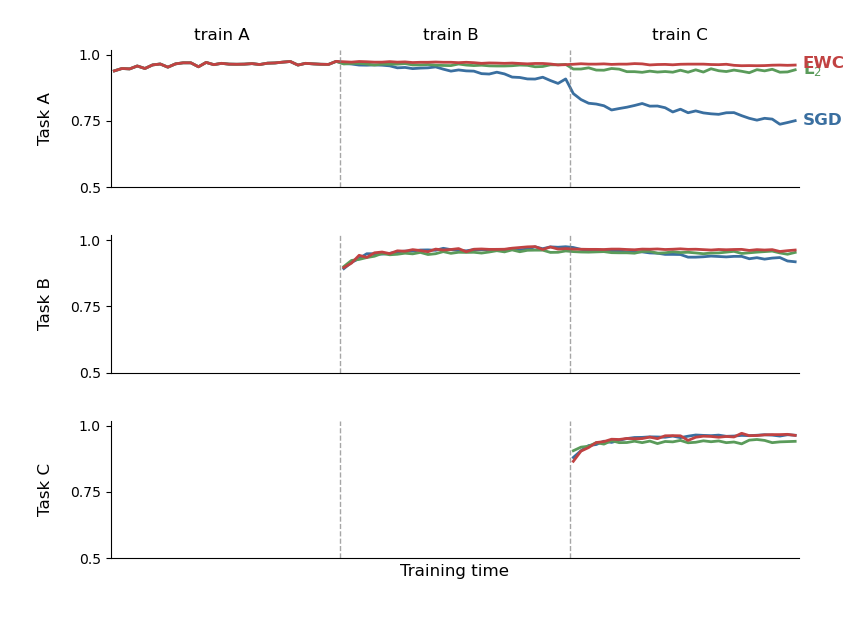
\includegraphics[width=\textwidth]{fig/EWC/ewc_paper_plot.png}
    \end{subfigure}
  \caption{}
  \label{fig:EWC_1}
\end{figure}
\noindent
Figure~\ref{fig:EWC_1} shows the test accuracy on three permuted-MNIST tasks
(\emph{A}, \emph{B}, \emph{C}) of a single MLP trained sequentially with
plain SGD, $L_2$ regularisation toward the previous parameters, and EWC.
Each row tracks one task across the entire training timeline; the dashed
vertical lines mark the transitions between training phases.
During \emph{train A}, all three methods reach comparable peak accuracy. As soon as
\emph{train B} begins, plain SGD overwrites the weights useful for $A$ and
its accuracy on $A$ drops sharply, illustrating catastrophic forgetting.
Uniform $L_2$ slows the drift but, treating every weight as equally
important, it must trade plasticity against stability and degrades on $A$
while only partially learning $C$. EWC instead anchors each parameter
$\theta_i$ to its post-$A$ value $\theta^{*}_{A,i}$ with a strength
proportional to the diagonal Fisher information
$F_i=\mathbb{E}_{(x,y)\sim\mathcal{D}_A}\!\big[(\partial_{\theta_i}\log
p_\theta(y\mid x))^2\big]_{\theta=\theta^{*}_A}$, estimated empirically by
averaging the squared per-parameter gradients of the log-likelihood over a
batch of $\mathcal{D}_A$ samples after training on $A$ (the Fishers from
successive tasks are summed). Because $F_i$ measures the local curvature
of task $A$'s loss, weights that matter for $A$ are held nearly fixed
while the rest are free to adapt, so EWC retains near-peak accuracy on $A$
and $B$ while still learning $C$.



\section{ Simple spike model}

\subsection{Definition of the model}

We consider the problem of recovering a low-rank signal hidden in a noisy symmetric matrix. In the spiked Wigner model, we observe a matrix $\rdmmat Y \in \R^{n\times n}$ consisting of a rank-one signal $\lambda \vect x \vect x^T$ with $\lambda \in \R$ and $\vect x \in \R^{n}$, corrupted by random noise $\rdmmat Z \in \R^{n \times n}$.

\begin{defn}[Spiked Wigner Model] \label{def:spiked-wigner}
Let $\lambda \in \mathbb{R}$ and let $\vect x \in \mathbb{R}^n$ be a signal vector satisfying \(\frac{\|\vect x\|^2}{n} \to 1\) as \(n \to \infty\). Let $\rdmmat Z$ be a symmetric Gaussian Wigner matrix, that is,
\begin{align}
Z_{ij} = Z_{ji}, \qquad Z_{ij} \overset{\mathrm{i.i.d.}}{\sim} \mathcal N(0,1)    \quad \text{for } 1\le i<j\le n,
\end{align}
and
\begin{align}
Z_{ii} \overset{\mathrm{i.i.d.}}{\sim} \mathcal N(0,1) \quad \text{for } 1\le i\le n.
\end{align}
\noindent
We define the spiked model as
\begin{align}
    \widetilde{\rdmmat Y} \;=\; \frac{\lambda}{\sqrt n}\,\vect u \vect u^T + \rdmmat W .
\end{align}
\end{defn}

\paragraph{Consistency between different normalizations}
\noindent
The model of Definition~\ref{def:spiked-wigner} can be rewritten in a more convenient normalization. Substituting $\rdmmat W = \sqrt{n}\,\rdmmat Z$, dividing by $\sqrt n$ and setting $\vect x = \vect u/\norm{\vect u}$ so that $\norm{\vect x}=1$, one obtains in the limit $n\to\infty$ (the full derivation is given in Appendix~\ref{adix:norm}):
\begin{equation}
    \rdmmat Y = \lambda \,\vect x \vect x^T + \rdmmat Z,
    \label{norm2}
\end{equation}
where $\|\vect x\|=1$ and $\rdmmat Z = \frac{1}{\sqrt n}\rdmmat W$. The two normalizations share the same asymptotic spectral behaviour, the eigenvalues of $\rdmmat Y$ and $\widetilde{\rdmmat Y}$ differing only by a $\frac{1}{\sqrt{n}}$ factor. For the rest of the report, we use the normalization of Eq.~\eqref{norm2}.

\subsection{Spectral method }\label{subsec:single-spike}

\subsubsection{Motivation for the spectral study of the observation $\mathbf{Y}$ } \label{section:1pike_gard_H}

The likelihood of $\rdmmat Y$ knowing the signal $x$ is given by :
\begin{equation}
    \text{P}(\rdmmat Y | \hat{\vect{x}}) \propto \text{exp}(-\frac{1}{2} \norm{\rdmmat Y - \lambda \hat{\vect{x}}\hat{\vect{x}}^T}^2_F)
\end{equation}
\noindent
Given the likelihood, the MLE loss is:
\begin{equation}
    \mathcal{L'} = -\frac{1}{2} \norm{\rdmmat Y - \lambda \hat{\vect{x}}\hat{\vect{x}}^T}^2_F
\end{equation}
\noindent
In practice, the MLE loss cannot be used since the signal-to-noise ration $\lambda$ is not known. The misspecified loss (MS) is then defined by:
\begin{equation}
    \mathcal{L}=-\frac{1}{2} \norm{\rdmmat Y - \hat{\vect{x}}\hat{\vect{x}}^{\top}}^2_F .
      \label{eq:MSloss}
\end{equation}
 The gradient update is given by :
 \begin{equation}
    {\hat{\vect{x}}}^{t+1} = {\hat{\vect{x}}}^t - \eta \vect{\nabla}_{{\hat{\vect{x}}}} \mathcal{L}
     \label{eq:GD}
 \end{equation}
\noindent
A direct component-wise computation (detailed in Appendix~\ref{adix:spectral-grad}) yields the gradient
\begin{equation}
    \vect{\nabla_{\hat{\vect{x}}}}\mathcal{L} = \rdmmat Y \hat{\vect{x}} - \norm{\hat{\vect{x}}}^2 \hat{\vect{x}}.
\end{equation}
\noindent
The Hessian of the loss $\mathcal{H}= \vect{\nabla}_{\hat{\vect{x}}}\vect{\nabla}_{\hat{\vect{x}}}^T \mathcal{L}$ follows immediately. Since with our normalization, for large dimensions $n$ we have $\norm{x} = 1$, it reads:
\begin{equation}
    \mathcal{H} = \vect{\nabla}_{\hat{\vect{x}}} [(\rdmmat Y  -\rdmmat I) \hat{\vect{x}}] = \rdmmat Y  -\rdmmat I \\
\end{equation}
with $\rdmmat I$ the identity matrix of dimensions $n \times n $. The hessian depends only on the observed matrix $\rdmmat Y$. And from eq.\ref{eq:GD}, the gradient descent update can be rewritten as:
\begin{equation}
    \hat{\vect{x}}^{t+1} = [\rdmmat I - \eta (\rdmmat Y - \rdmmat I)] \hat{\vect{x}}^t = [\rdmmat I - \eta \mathcal{H}] \hat{\vect{x}}^t
\end{equation}
Since the Hessian is constant and symmetric, each gradient descent step applies the same linear operator to $\mathbf{x}$, progressively amplifying its component along the eigenvector of $\rdmmat Y - \rdmmat I$  associated with the largest eigenvalue. Gradient descent therefore converges to the leading eigenvector of $\rdmmat Y - \rdmmat I$ , which coincides with the leading eigenvector of $\rdmmat Y$ itself.
Minimizing the MS loss is thus equivalent to performing a spectral decomposition of $\rdmmat Y$, and both approaches yield the same solution.



\subsubsection{ BBP transition and Spectral method} 

The goal is to recover the hidden vector $\vect x$ from the observation $\rdmmat Y$. The possibility of recovering the signal is governed by the signal-to-noise ratio parameter $\lambda$. When $\lambda$ is sufficiently large, an eigenvalue corresponding to the signal separates from the bulk of the spectrum. This phenomenon is known as the \emph{BBP phase transition} and indicates that the signal becomes detectable through spectral methods.
\noindent
Before describing this transition, it is important to recall that the global distribution of the eigenvalues of a Wigner matrix admits a deterministic limit.

\begin{theo}[Semicircle Law]\label{thm:semi-circle}
Let $\lambda_1(Y),\dots,\lambda_n(Y)$ denote the eigenvalues of $\rdmmat Y$. The empirical spectral distribution
\begin{align}
\hat{\mu}_Y := \frac{1}{n}\sum_{i=1}^n \delta_{\lambda_i(Y)}
\end{align}
converges weakly almost surely as $n \to \infty$ to the semi-circle distribution with density
\begin{align}
    \rho_{sc}(x) := \frac{1}{2\pi}\sqrt{4-x^2}\,\mathbf{1}_{|x|\le 2}.
\end{align}
\end{theo}


\noindent
Furthermore, spectral analysis does not only yield eigenvalues distribution, or equivalently, it does not only give a certification about whether one can recover a signal or not. 
\noindent
While one can obtain the threshold by computing the top eigenvalue of $\rdmmat Y$, the top eigenvector associated corresponds to an estimator $\hat {\vect x}$ of $\vect x$. 
\noindent
To know if this is a good estimation, We define the overlap: 
\begin{equation}
    m_n = \lvert \langle \hat{\vect x} 
     , \vect x\rangle \rvert = \rvert\sum_{i=1}^n \hat{x}_i x_i \rvert \, .
    \label{eq:overlap_u}
\end{equation}
\noindent
One can think about the overlap as the alignment between the estimator and the signal. If the estimator is good, they should be aligned and the overlap should go to $1$. Otherwise, if the estimator is randomly chosen, it is most likely orthogonal to the signal in high dimension and the overlap should go to $0$.
\medskip 

\begin{theo}[BBP transition]\label{thm:bbp}
Let $\hat{\vect x}$ be the top eigenvector of $\rdmmat Y$ associated to the eigenvalue $\lambda_{\max}$. Additionally, $\hat{\vect x}$ is normalized so that $\|\hat{\vect x}\|/\sqrt n\to1$. Then, as $n\to\infty$, the largest eigenvalue satisfies
\begin{align}
\lambda_{\max}(Y)\xrightarrow{\mathrm{a.s.}}
\begin{cases}
2 & \text{if } \lambda \le 1,\\[0.3em]
\lambda+\lambda^{-1} & \text{if } \lambda > 1,
\end{cases}
\end{align}
and the squared overlap between $\hat{\vect x}$ and the spike direction $\vect x$ satisfies
\begin{align}
    m_n
    %
    \xrightarrow{\mathrm{a.s.}}
    %
    m := \begin{cases}
        0 & \text{if } \lambda \le 1,\\[0.3em]
        \sqrt{1-\lambda^{-2}} & \text{if } \lambda > 1.
    \end{cases}
\end{align}
In particular, weak recovery by PCA is possible if and only if \(\lambda>1\).
\end{theo}




\subsection{Numerical experiments of BBP}

\subsubsection{Simple plots of eigenvalue distribution}
We first try to plot our Wigner matrix, with no spikes and different values of $n = 1000$, then with a constant value of $n$ and with different spikes. Each time, we numerically compute the maximal eigenvalue found and plot it in red. We also plot the Wigner Semi-Circle to show the bulk's distribution follows it. These first results are presented in Fig. \ref{first_plot1}.

\begin{figure}[ht] 
\noindent\hspace*{-1.5cm}
   \begin{subfigure}{0.6\textwidth}
        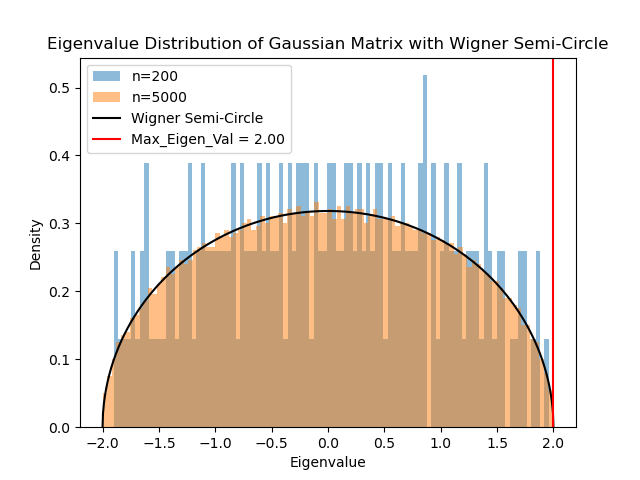
\includegraphics[width=\textwidth]{fig/no_spike.png}
                \caption{}

    \end{subfigure}
    \begin{subfigure}{0.6\textwidth}
    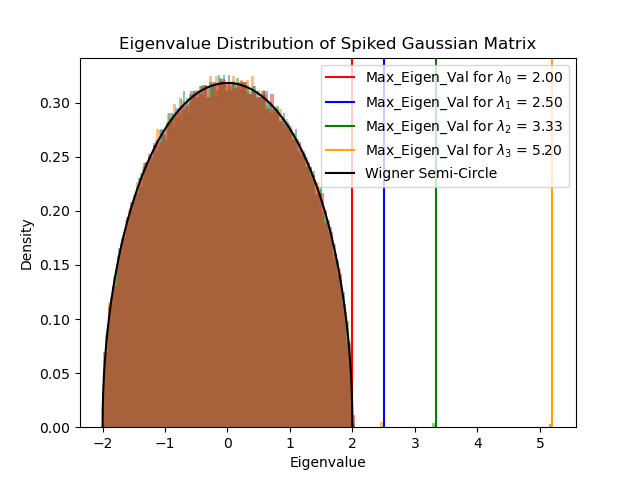
\includegraphics[width=\textwidth]{fig/many_spikes.png}
            \caption{}

    \end{subfigure}
  \caption{a) Distribution of the eigenvalues of $\rdmmat W$ for two matrix sizes: n = 200 and n = 5000, with Wigner Semi-Circle and the maximum eigenvalue found.
  b) Distribution of the eigenvalues of $\rdmmat Y$ for n = 1000 and different values of $\lambda = 1, 2, 3, 5$, with Wigner Semi-Circle and maximum eigenvalue found (each time).
  }
  \label{first_plot1}
\end{figure}
\noindent
Fig. \ref{first_plot1}a) show for higher values of $n$, the Wigner distribution is a way better approx, wich was expected. Fig. \ref{first_plot1}b) shows that when plotting the distribution of a spiked Wigner matrix with $\lambda \leq1$, the maximal eigenvalue is the same as before (it is 2). But when $\lambda > 1$ the maximal eigenvalue is located where the BBP transition theorem \ref{eq:2spikes} predicts it. So for $\lambda<1$ the bulk swallows the spike.
\noindent
We now try to see, what is the maximal eigenvalue as a function of lamba, to check if, for $n=1000$, our BBP theorem is indeed in accordance with what we can compute.

\begin{figure}[ht] 
\centering
    \begin{subfigure}{0.6\textwidth}
    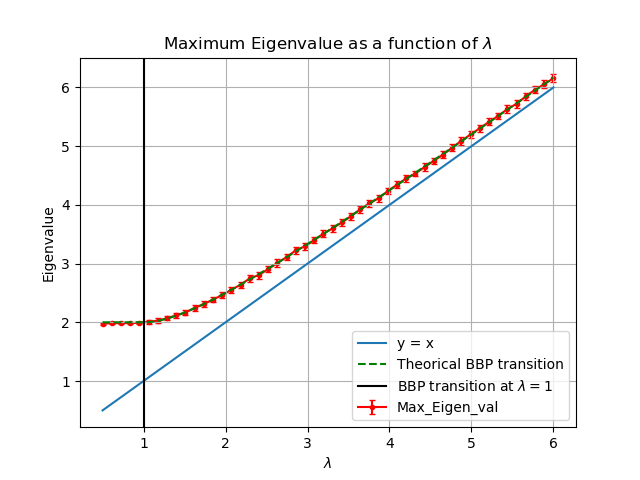
\includegraphics[width=\textwidth]{fig/BBP_transi_obs.png}
            \caption{}

    \end{subfigure}
  \caption{Maximal eigenvalue computed and theoritical as a function of $\lambda$, with $y = x$, for $n = 1000$.}
  \label{second_plot}
\end{figure}
\noindent
Fig.\ref{second_plot} shows the maximal eigenvalue we compute for a single spike indeed follows the BBP theory. We can observe the value of the theoretical maximal observable eigenvalue is always the same as the maximal eigenvalue we observe. We also see the $\frac{1}{\lambda}$ dependence very well especially for large $\lambda$.

\subsubsection{Overlaps}
The obtained empirical overlap $m_n$ and the theoretical asymptotic prediction $m$ as function of $\lambda$ is given in Fig.\ref{fig: overlap1spike}.


\begin{figure}[ht]
    \centering
    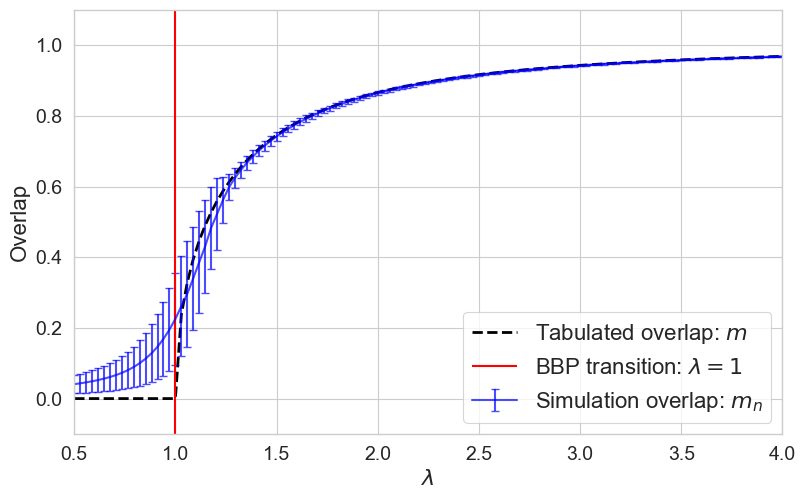
\includegraphics[width=0.7\textwidth]{fig/overlap_1spike.png}
    \caption{Exercise 3.2: Empirical overlap $m_n$ and the theoretical asymptotic prediction $m$ vs. $\lambda$. We have $n = 2000$, and the simulated overlap $m_n$ is the mean overlap over 30 simulations with error given by its standard deviation.}
    \label{fig: overlap1spike}
\end{figure}

\begin{rem}\label{rem:bbp} \leavevmode
\begin{itemize}
    \item \textbf{Choice of the prior:} We mentioned the choice of the prior in the previous exercise. Indeed, this results remains for other prior that respects some assumptions. It should be centred, variance $1$ and a finite fourth moment (which avoids a fat tail distribution). 
    \item \textbf{Equivalence between methods:} For this simple spiked matrix, most of the methods are equivalent for the threshold. Indeed, we consider a spectral decomposition of the observation $\rdmmat Y$ but there exists many others. (i) One could define a loss and apply the well known\textit{ Gradient Descent} method. This method gives the same threshold and same overlaps performance. (ii) One could also think about Bayesian methods and define a smart algorithm called \textit{Approximate Message Passing} that we will see later on. This algorithm yields the same recovery threshold but better overlap performances; one could improve the spectral method performances by optimizing the norm of the estimator, but it does not bring any bonus to the story.

    However, A complete analysis is not the main focus but it is worth mentioning that for some priors this equivalence between methods fails (like Gaussian, Rademacher and others). For instance, if we consider a sparse prior, such as: $\vect x \sim \epsilon\, \mathcal{R}(1/2) + (1-\epsilon)\delta_0$ with $\epsilon\in [0,1]$ and $\delta_0$ the null prior (in other words, a prior that gives $0$ most of the time and a Rademacher the rest of the time). In that case, AMP outperforms spectral method and even more interesting there is a phase where the information is available but no algorithm can recover it. This phase is often called "HARD". See \cite{Lesieur_2017}.
\end{itemize}
\end{rem}

\section{Spiked Model for multi-task setting}\label{subsec:multi-spiked}

The multi-task problem on real datasets can be theoretically studied through the lens of the multi-task spiked model. This model offers a clean mathematical framework that captures the key structure of high-dimensional data shared across multiple tasks. In this section, we introduce the spiked model in the multi-task setting and draw parallels between its assumptions and the properties of real-world datasets. This connection allows us to use the spiked model as a simple yet powerful tool to better understand the behavior of multi-task learning in practice.

\subsection{Definition of the Spiked Model for multi-task setting}
We assume that the tasks are not completely independent, in other words, we reasonably assume correlations between tasks. This leads to the following definition:

\begin{defn}[Multi-Task Spiked Wigner Model]\leavevmode\\
    Let $\lambda_1, \lambda_2 \in \R$ the signal-to-noise ratio per task and $\vect x_1, \vect x_2 \in \R^n$, with $\norm{\vect x_1} = \norm{\vect x_2} = 1$ the correlated signals per task from a multivariate Gaussian Prior:
    \begin{align}
        \forall i \in[n]\,,\; \para{x_{1,i}\;\; x_{2,i}}^T \overset{\mathrm{i.i.d.}}{\sim} \mathcal{N}(\vect 0, \mat C)\, ,\quad\mathrm{with}\quad \mat C := \begin{pmatrix}
            1 & \rho \\
            \rho & 1 
        \end{pmatrix}\,,\quad \mathrm{and}\quad \rho \in [0,1]\,.
    \end{align} 
    We define independent  Gaussian noises $\rdmmat Z_1$ and $\rdmmat Z_2$, namely:
    \begin{align}
        \forall (t,i,j) \in\{1,2\}\times[n]^2 \,, \; Z_{t,ij} = Z_{t,ji} \overset{\mathrm{i.i.d.}}{\sim} \mathcal{N}\bigg(0,\frac{1}{n}\bigg) .
    \end{align}
    We write the multi-spiked model as:
    \begin{align}
        \rdmmat Y_1 \, = \, \lambda_1 \vect x_1 \vect x_1^T + \rdmmat Z_1 \, , \\
        \rdmmat Y_2 \, = \, \lambda_2 \vect x_2 \vect x_2^T + \rdmmat Z_2 \, .
    \end{align}
    \noindent
    Our observation is then:
    \begin{equation}
    \rdmmat Y := \alpha \rdmmat Y_1 + \sqrt{1-\alpha^2} \cdot \rdmmat Y_2
    \label{eq:2spikes}
    \end{equation}
    \noindent
    with $ \alpha$ the importance factor, giving how important the task $i = 1,2$ is.
\end{defn}


\noindent
The contrast between the multi-modal model and the multi-task model lies in the philosophy of the estimation. For multi-modal models, since each spike is seen as a modality to infer, there will be as many estimators as modalities, and the model will try to benefit from correlations to best infer all the modalities. However, the multi-task model keeps only one estimator that needs to remain "good" on all the tasks that are presented. In GD optimization, the tasks are seen sequentially in time for practical reasons, but here we will not restrict ourselves to sequential inference. Thus, we need to define what it means to have an estimator that remains "good" on all the tasks: what is the appropriate measure? EWC defines an error for training but not for testing!



\subsection{Naive Spectral Method}

\begin{defn}(Multi-Task MSE)\leavevmode\\
    For given observations $\rdmmat Y_1 \in \R^{n\times n}$ and $\rdmmat Y_2 \in \R^{n \times n}$ and an estimator $\hat{\vect x} \in \R^n$, we define the MS Loss as:
    \begin{align}
        \mathcal{L}_{\mathrm{MSE}}(\vect x) := \alpha \norm{\rdmmat Y_1 - \vect x\vect x^T}^2_F + \sqrt{1-\alpha^2} \norm{\rdmmat Y_2 - \vect x\vect x^T}^2_F\,,\quad \mathrm{with}\quad \alpha \in [0,1]
    \end{align}
The overlap for each signal is defined as in eq.~\ref{eq:overlap_u}.
\end{defn}
\noindent
A computation analogous to the single-spike case (detailed in Appendix~\ref{adix:naive-grad}) gives the gradient $\vect{\nabla} \mathcal{L}_{\mathrm{MSE}}(\vect x) = \alpha (\rdmmat Y_1 - \rdmmat I)\vect x + \sqrt{1-\alpha^2} (\rdmmat Y_2 - \rdmmat I)\vect x$ and the Hessian
\begin{equation}
    \mathcal{H} = \alpha \rdmmat Y_1 + \sqrt{1-\alpha^2} \rdmmat Y_2 - \rdmmat I ( \alpha + \sqrt{1-\alpha^2}) = \rdmmat Y - \rdmmat I ( \alpha + \sqrt{1-\alpha^2}).
\end{equation}
\noindent
Since the Hessian depends only on $\rdmmat Y$, the equivalent spectral method of Sec.~\ref{subsec:single-spike} is studying the top eigenvalue of $\rdmmat Y$ and our estimator $\hat{\vect{x}}$ for the tasks $\rdmmat Y_1$ and $\rdmmat Y_2$ is given by the top eigenvector of the observation $\rdmmat Y$.



\noindent
If there exists an equivalence between methods for the single spike model, it is absolutely not true for several correlated spikes. There is no reason why this method should perform good, it is just an intuitive method designed from the loss. For instance, this break of equivalence between methods is what happens in multi-modal inference. \cite{Keup_2025, mergny2025spectralthresholdscorrelatedspiked, tabanelli2025computationalthresholdsmultimodallearning}


\subsection{Numerical analysis for the spectral method}
Given our output $\rdmmat Y$ , we analyse the recovered signal obtained for both spikes 1 and 2. For each signal, our estimator of the signal ($\hat{u}_i$) is given by the eigenvector of the $\rdmmat Y$ matrix corresponding to the signal eigenvalue. So for the two spikes, their estimator will either be the eigenvector of the highest eigenvalue ($v_1$) or the one of the second biggest eigenvalue ($v_2$). 

\subsubsection{Observation of two correlated spikes}
We now observe how the two maximal eigenvalues appear for different values of $\rho$ and $ \alpha$.
\begin{figure}[ht] 
\centering  
   \begin{subfigure}[t]{0.48\textwidth}
        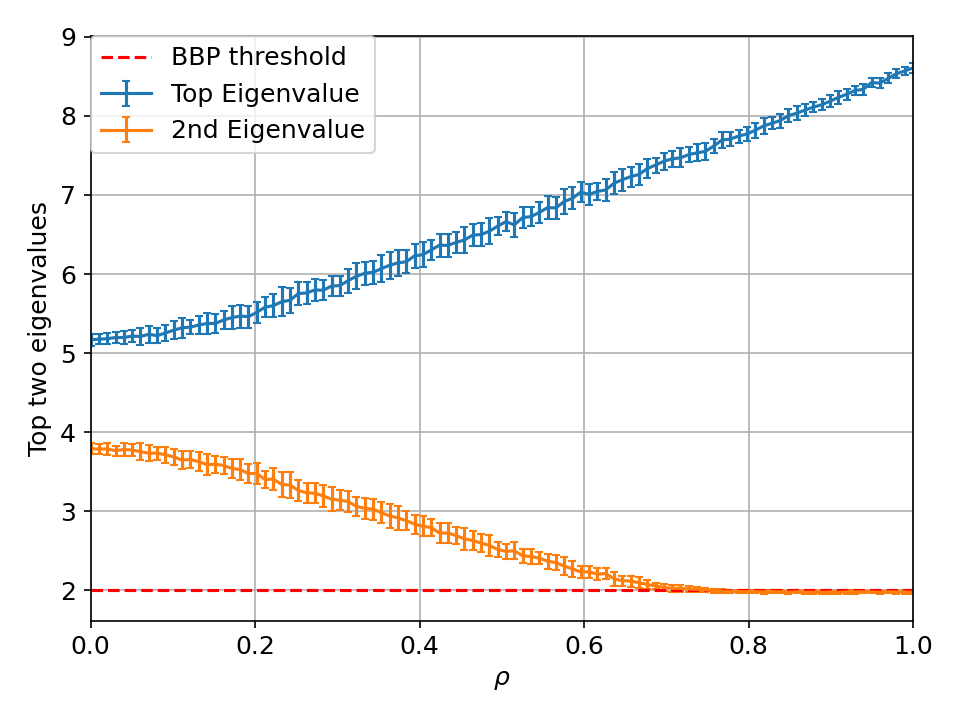
\includegraphics[width=\textwidth]{fig/Two_Spiked_Wigner_Top_Eigenvalues_alpha_0.71.png}
        \caption{}
    \end{subfigure}
    \hfill
    \begin{subfigure}[t]{0.48\textwidth}
        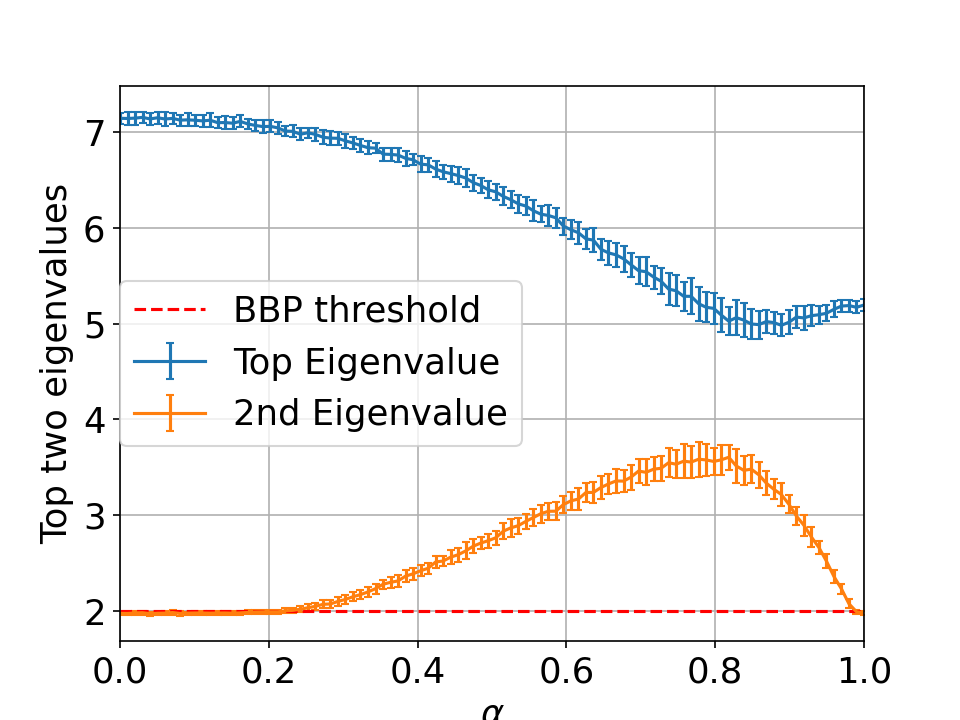
\includegraphics[width=\textwidth]{fig/Two_Spiked_Wigner_Top_Eigenvalues_rho_0.2.png}
        \caption{}
    \end{subfigure}
    \caption{Analysis of Spiked Wigner Model Eigenvalues. Two maximal eigenvalues for different values of $\alpha$. Taken as an average over 50 spikes. For a fixed value of $\rho = 0.2$.Two maximal eigenvalues for different values of $\rho$. Taken as an average over 50 spikes. For a fixed value of $\alpha = \sqrt{0.5} \approx 0.71$ (equally weighted spikes).}
    \label{first_plot}
\end{figure}
\noindent
Plots are computed using $\lambda_1 = 5$ and $\lambda_2 = 4$ as spikes values, and a matrix size of $n = 500$. The maximal two eigenvalues are found numerically. Fig . \ref{first_plot} a) shows that as correlation increases, the spike corresponding to the greater eigenvalue moves away from the bulk, as the one with the lower eigenvalue (the second greatest) moves towards the bulk and becomes indistinguishable from it. Fig. \ref{first_plot} b) shows that as $\alpha$ increases, the first spike ($i = 1$) gains significance in the observation, while the second spike ($i = 2$) loses significance in the observation. At $\alpha = 0.71$, corresponding to equally weighted spikes, the trends invert, with the first spike having more significance than the second one.

\subsubsection{Overlap analysis}
The overlaps between both signals $\vect x_1$, $\vect x_2$ and our estimator $\hat{\vect{x}}$ (the top  eigenvector of $\rdmmat Y$), are computed as function of different parameters. 

\paragraph{Standard conditions}
Taking $\lambda_2 >1$ so that we are not in the BBP transition for the second spike $\vect x_2 \vect x_2^T$  and a correlation factor of zero, $\rho = 0$, we then have 2 independent spikes. 

\noindent
In this case, given eq.(\ref{eq:2spikes}), the two signals contribute equally to the matrix when their effective strengths match:
\begin{equation}
    \alpha_*  \cdot \lambda_1 = \sqrt{1 - \alpha_* ^2} \cdot \lambda_2  \quad \implies \quad \alpha_* = f(\lambda_1) = \sqrt{\frac{(\frac{\lambda_2}{\lambda_1})^2}{1+(\frac{\lambda_2}{\lambda_1})^2}}
    \label{eq:alpha=f(k1)}
\end{equation}
\noindent
The Fig.\ref{fig:m_alpha_vs_lambda1_rho0} shows the obtained overlaps for both signals as function of $\alpha$ and $\lambda_1$ and the line defined by eq.\ref{eq:alpha=f(k1)}.

\begin{figure}[ht] 
   \begin{subfigure}{0.5\textwidth}
        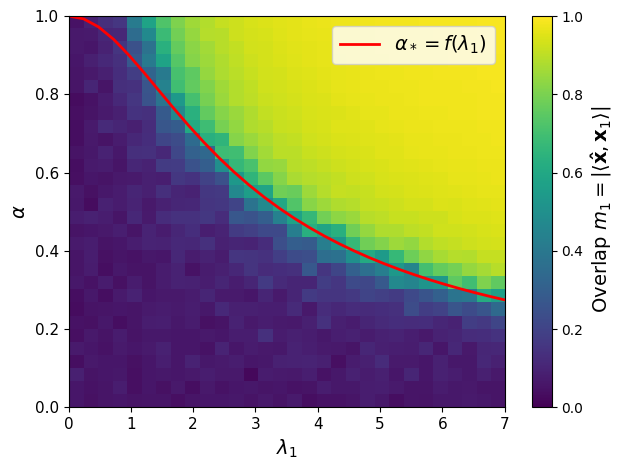
\includegraphics[width=\textwidth]{fig/m2spikes/alpha_vs_lambda1/m1_rho0.png}
         \caption{}
    \end{subfigure}
    \begin{subfigure}{0.5\textwidth}
    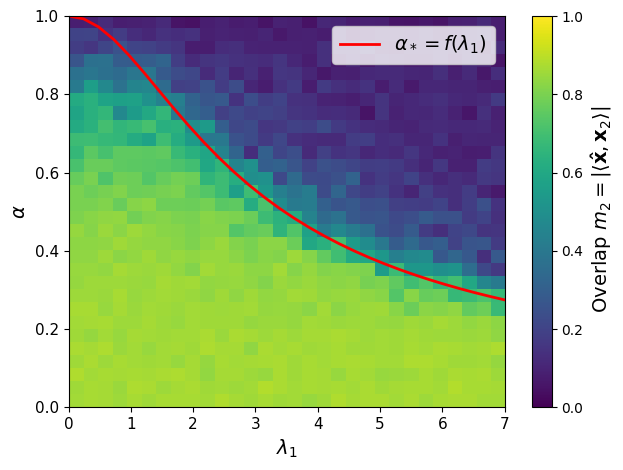
\includegraphics[width=\textwidth]{fig/m2spikes/alpha_vs_lambda1/m2_rho0.png}
            \caption{}
            \label{fig:m2_alpha_vs_lambda1}
    \end{subfigure}
  \caption{\centering Overlaps $m$ as function of the importance factor $\alpha$ and the value of $\lambda_1$ for (a) the first signal $x_1$, (b) the second $x_2$. With the fixed parameters:  $\lambda_2=2$, $\rho = 0$. 
    The red line is the line of eq.\ref{eq:alpha=f(k1)} with $\lambda_1 >1$. The simulation is done for dimension of the spikes $n=200$ and the overlap is computed as the mean overlap over 10 simulations.}
    \label{fig:m_alpha_vs_lambda1_rho0}
\end{figure}

\noindent
 In the absence of correlation between the two spikes, the estimator $\hat{\mathbf{x}}$ cannot recover both signals simultaneously. As expected, the top eigenvector aligns with the signal associated with the largest eigenvalue. This is reflected in the figure by the fact that only one overlap is non-zero at a time.
\noindent
For $\lambda_i > 1$, recovery of signal $i$ occurs only when its strength exceeds that of the competing signal. Conversely, the overlap with the weaker signal remains zero, since no information about it is contained in the estimator. Furthermore, the transition line defined by  $\alpha_*$, 
is visible in the figure as the line where the dominant signal switches.
\noindent
For $\lambda_1 < 1$, the first spike lies below the BBP threshold and does not produce an outlier eigenvalue, hence it cannot be recovered.
\noindent\noindent
Finally, as $\lambda_1 \to 0$, $\alpha_* \to 1$, so the contribution of the second signal vanishes, making its recovery impossible. As shows Fig. \ref{fig:m2_alpha_vs_lambda1}, its overlap with the estimator becomes zero. 

\\
Now fixing $\alpha$ so that both signals have the same importance ($\alpha = \sqrt{1-\alpha^2}$ ), the overlap for both signal is studied varying $\lambda_1$ and the $\lambda_2$.



The overlap for both signal is studied varying the correlation $\rho$ and the $\lambda_1$.
\begin{figure}[ht] 
   \begin{subfigure}{0.5\textwidth}
        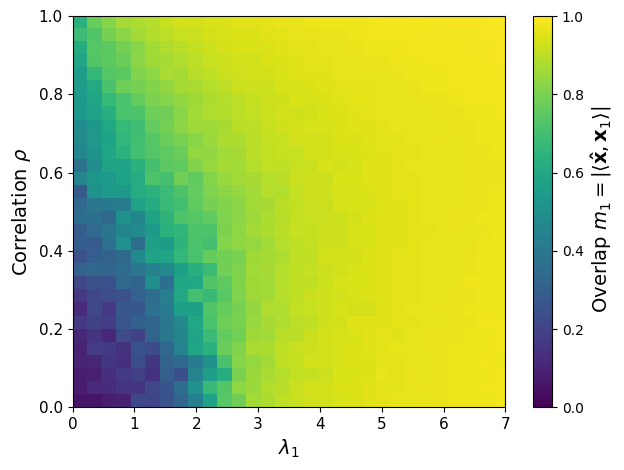
\includegraphics[width=\textwidth]{fig/m2spikes/standard_cond/m1_rho_vs_lambda1__alphasqrt05_lambda2_3.png}
                \caption{}
    \end{subfigure}
    \begin{subfigure}{0.5\textwidth}
    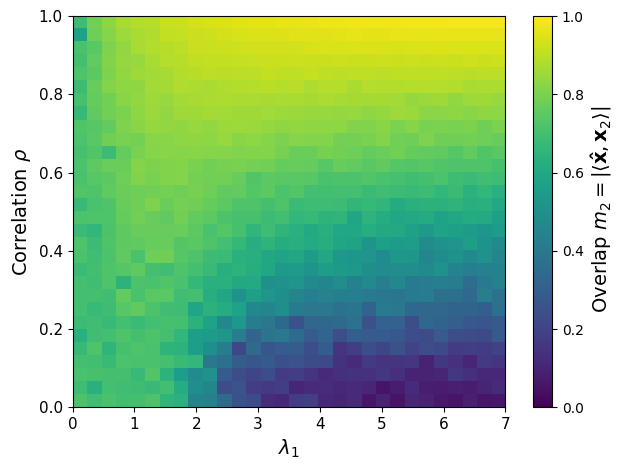
\includegraphics[width=\textwidth]{fig/m2spikes/standard_cond/m2_rho_vs_lambda1__alphasqrt05_lambda2_3.png}
            \caption{}
    \end{subfigure}
  \caption{\centering Overlaps $m$ as function of the correlation $\rho$ and the value of $\lambda_1$ for (a) the first signal $x_1$, (b) the second $x_2$. With the fixed parameters:  $\lambda_2=2$, $\alpha= \sqrt(0.5)$. The simulation is done for dimension of the spikes $n=200$ and the overlap is computed as the mean overlap over 10 simulations.}
  \label{fig:m_rho_vs_lambda1}
\end{figure}

For small correlation $\rho \leq 0.3$, the same phenomenon as in Fig. \ref{fig:m_alpha_vs_lambda1} is observed. Since both signals have the same importance, for $\lambda_1 < \lambda_2$, only the second signal is recovered and no information of the first signal is contained in our estimator $\hat{x}$, the opposite is observed when $\lambda_1$ becomes greater than $\lambda_2$.

When the correlation increases, the two signals have informations in common, and both signals are partially recovered. For a high correlation, $\rho \geq 0.6$, both signals are recovered, even for $\lambda_1 \leq 1$, since $\lambda_2 \geq 1$ the informations of the first signals are also in the second signals and so our estimator describes well both signals.

\begin{figure}[H] 
   \begin{subfigure}{0.5\textwidth}
        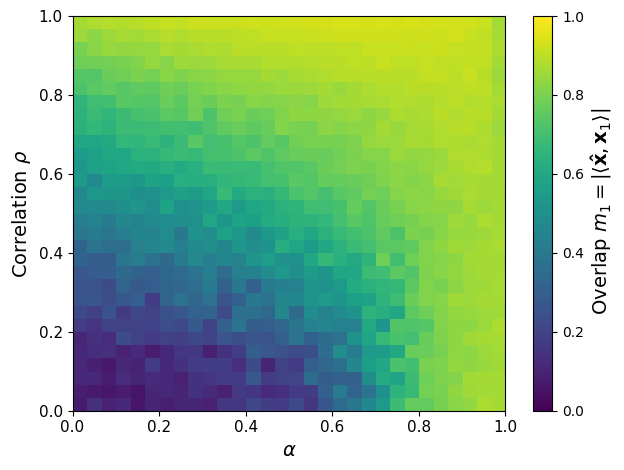
\includegraphics[width=\textwidth]{fig/m2spikes/standard_cond/m1_rho_vs_alpha__lamnda1_lambda2_3.png}
                \caption{}
    \end{subfigure}
    \begin{subfigure}{0.5\textwidth}
    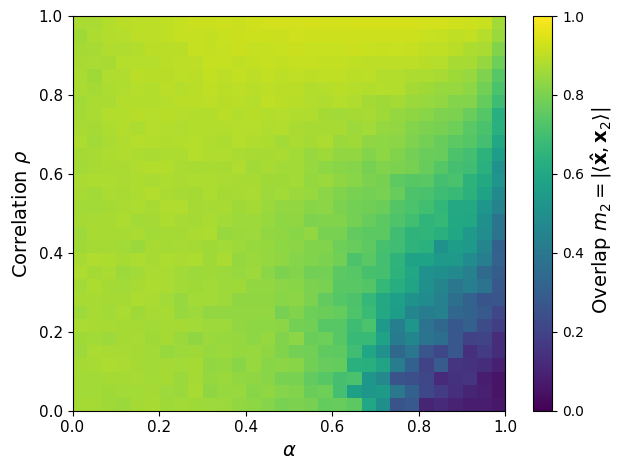
\includegraphics[width=\textwidth]{fig/m2spikes/standard_cond/m2_rho_vs_alpha__lamnda1_lambda2_3.png}
            \caption{}
    \end{subfigure}
  \caption{\centering Overlaps $m$ as function of the correlation $\rho$ and the importance factor $\alpha$ for (a) the first signal $x_1$, (b) the second $x_2$. With the fixed parameters:  $\lambda_1 = \lambda_2=2$. The simulation is done for dimension of the spikes $n=200$ and the overlap is computed as the mean overlap over 10 simulations.}
  \label{fig:m_rho_vs_lambda1}
\end{figure}

When $\lambda_1 > \lambda_2$, the information about $\vect{x}_2$ is split between the two leading eigenvectors $v_1$ and $v_2$: the correlation is large enough to inject part of the information about $\vect{x}_1$ into $v_1$, but not sufficient for $v_1$ alone to carry the full signal of $\vect{x}_2$. At lower correlation, all information about $\vect{x}_2$ concentrates in $v_2$.

Above a critical correlation threshold, the information from \emph{both} spikes concentrates in the single leading eigenvector; a single eigenvector then describes both signals simultaneously.
    




\subsubsection{Observation of the phase transition }
Now, I will try to plot a phase diagram, trying to identify the shape of the different recovery region for $m_1$ and $m_2$.

\begin{figure}[ht]
    \centering % Centers the entire block of images
    \begin{subfigure}{0.33\textwidth}
        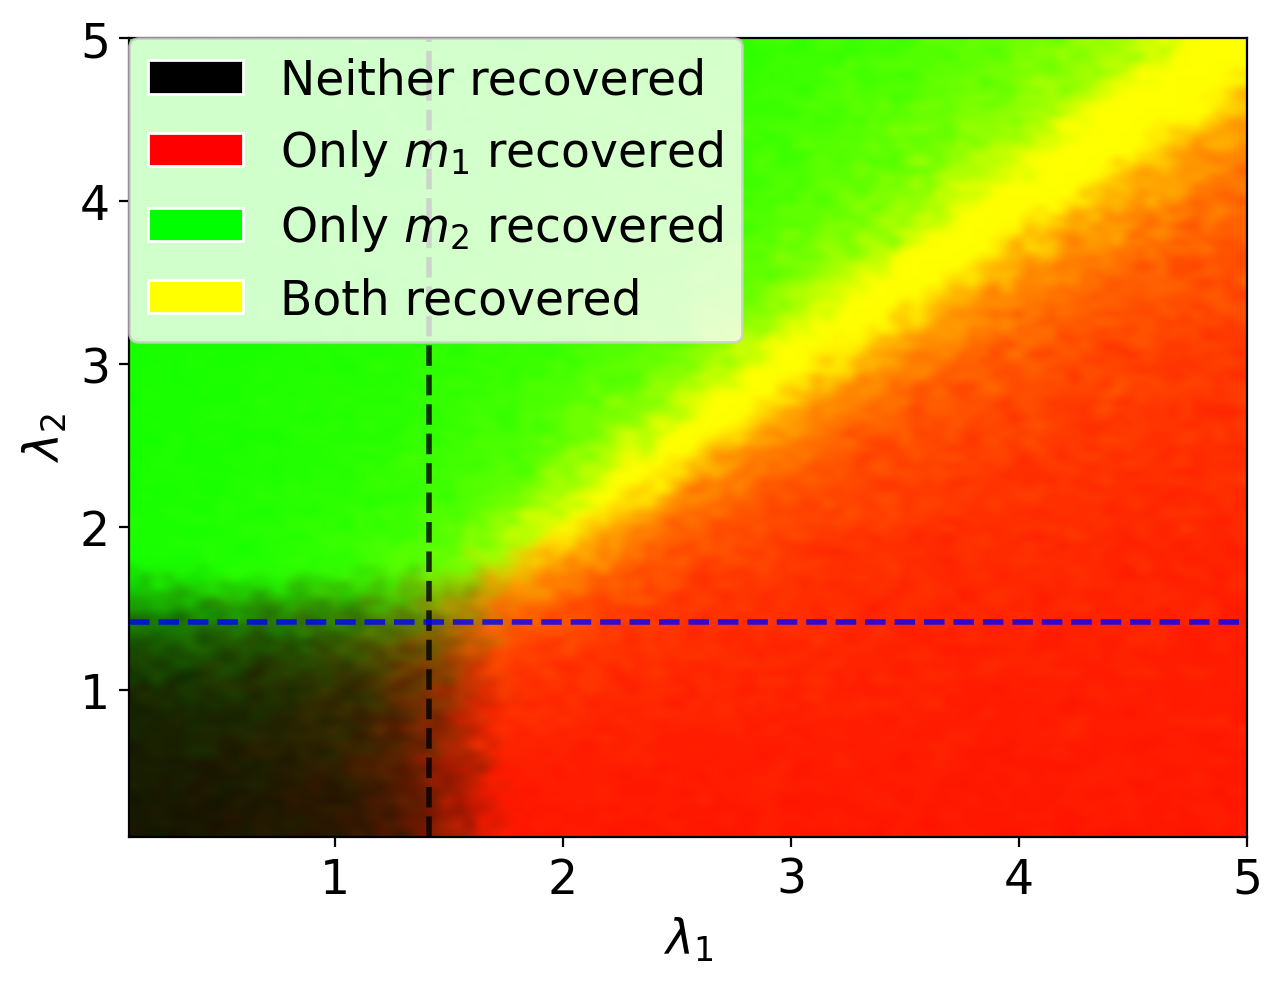
\includegraphics[width=\textwidth]{fig/fig_phase_transition/Phase_Diagram_alpha=0.71_rho=0.00.png}
        \caption{}
    \end{subfigure}\hfill % \hfill pushes the subfigures apart evenly
    \begin{subfigure}{0.33\textwidth}
        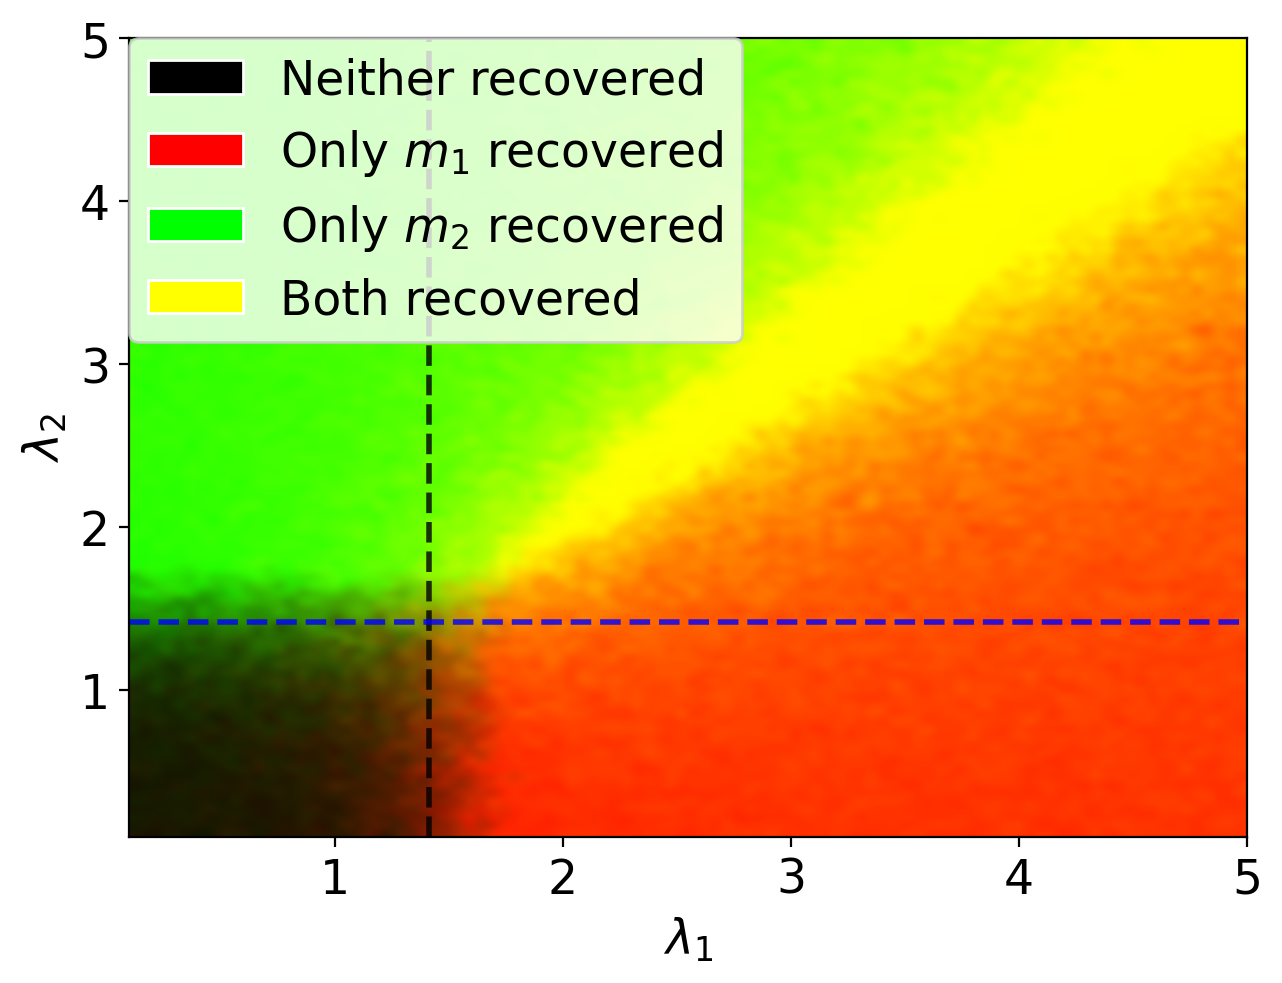
\includegraphics[width=\textwidth]{fig/fig_phase_transition/Phase_Diagram_alpha=0.71_rho=0.10.png}
        \caption{}
    \end{subfigure}\hfill
    \begin{subfigure}{0.33\textwidth}
        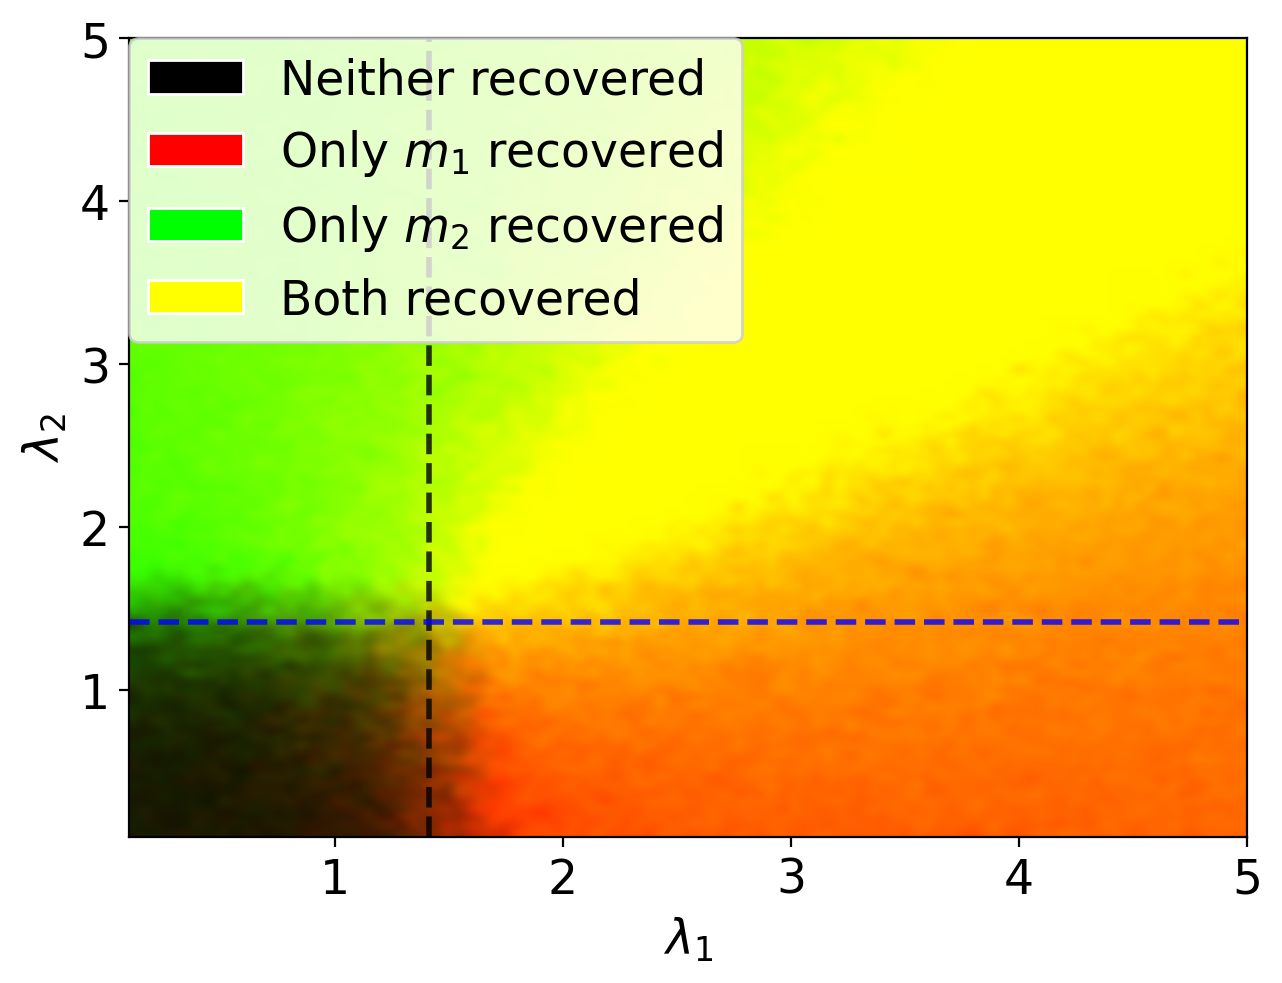
\includegraphics[width=\textwidth]{fig/fig_phase_transition/Phase_Diagram_alpha=0.71_rho=0.20.png}
        \caption{}
    \end{subfigure}
    \begin{subfigure}{0.32\textwidth}
        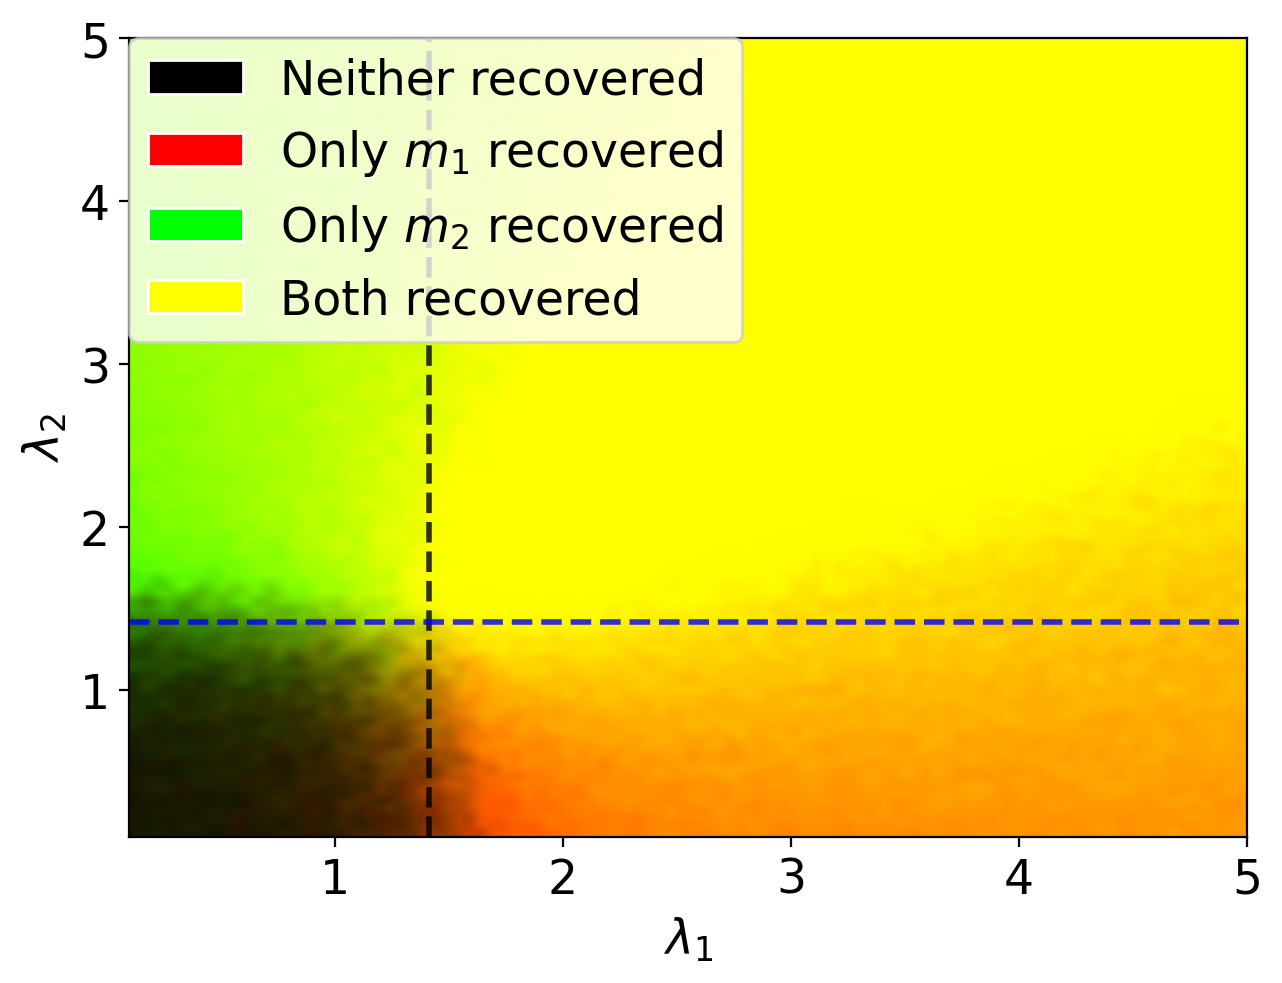
\includegraphics[width=\textwidth]{fig/fig_phase_transition/Phase_Diagram_alpha=0.71_rho=0.30.png}
        \caption{}
    \end{subfigure}\hfill
    \begin{subfigure}{0.32\textwidth}
        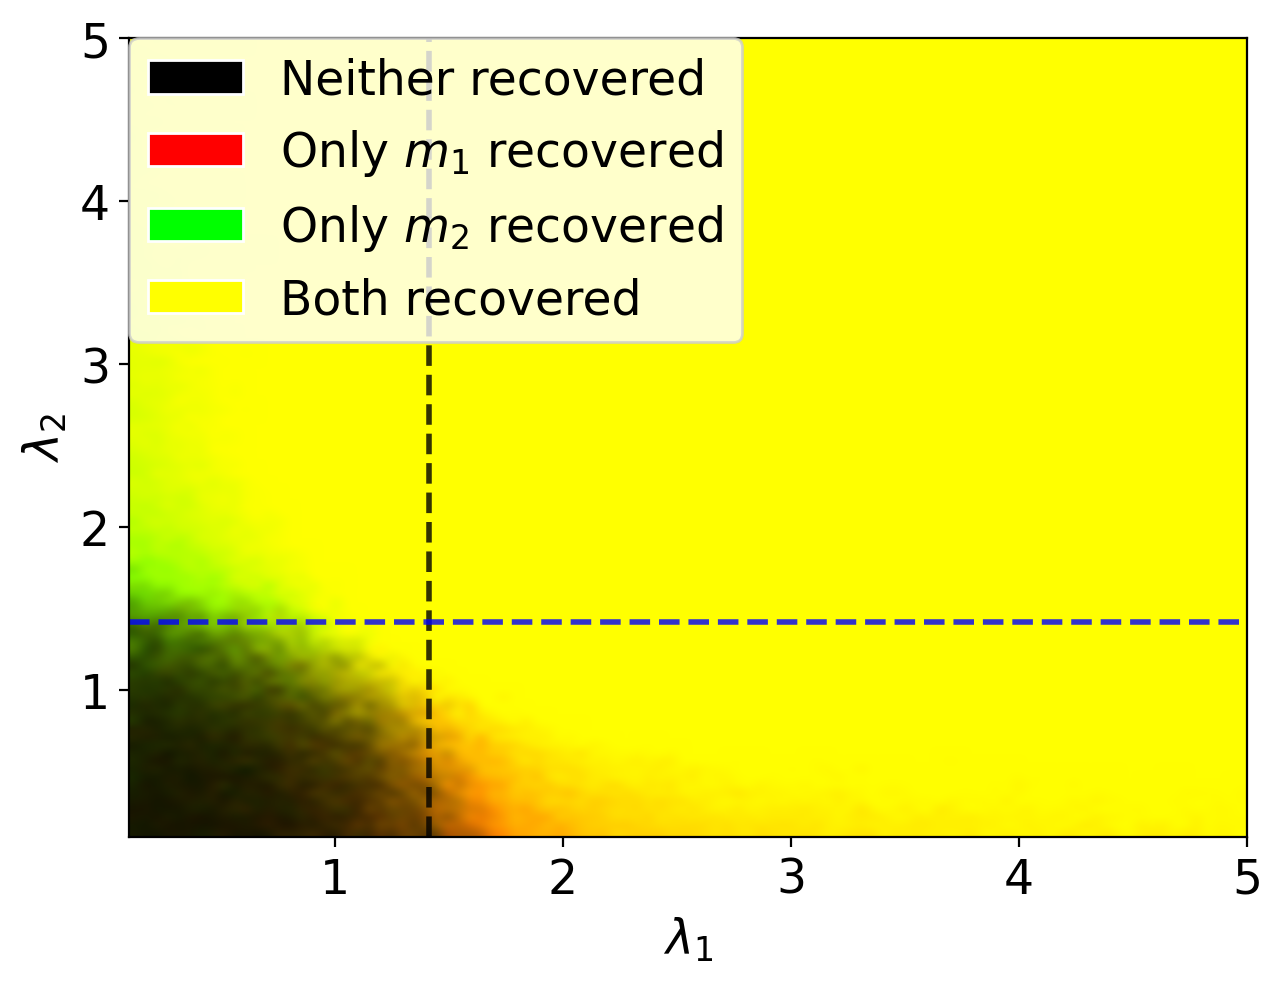
\includegraphics[width=\textwidth]{fig/fig_phase_transition/Phase_Diagram_alpha=0.71_rho=0.50.png}
        \caption{}
    \end{subfigure}\hfill
    \begin{subfigure}{0.32\textwidth}
        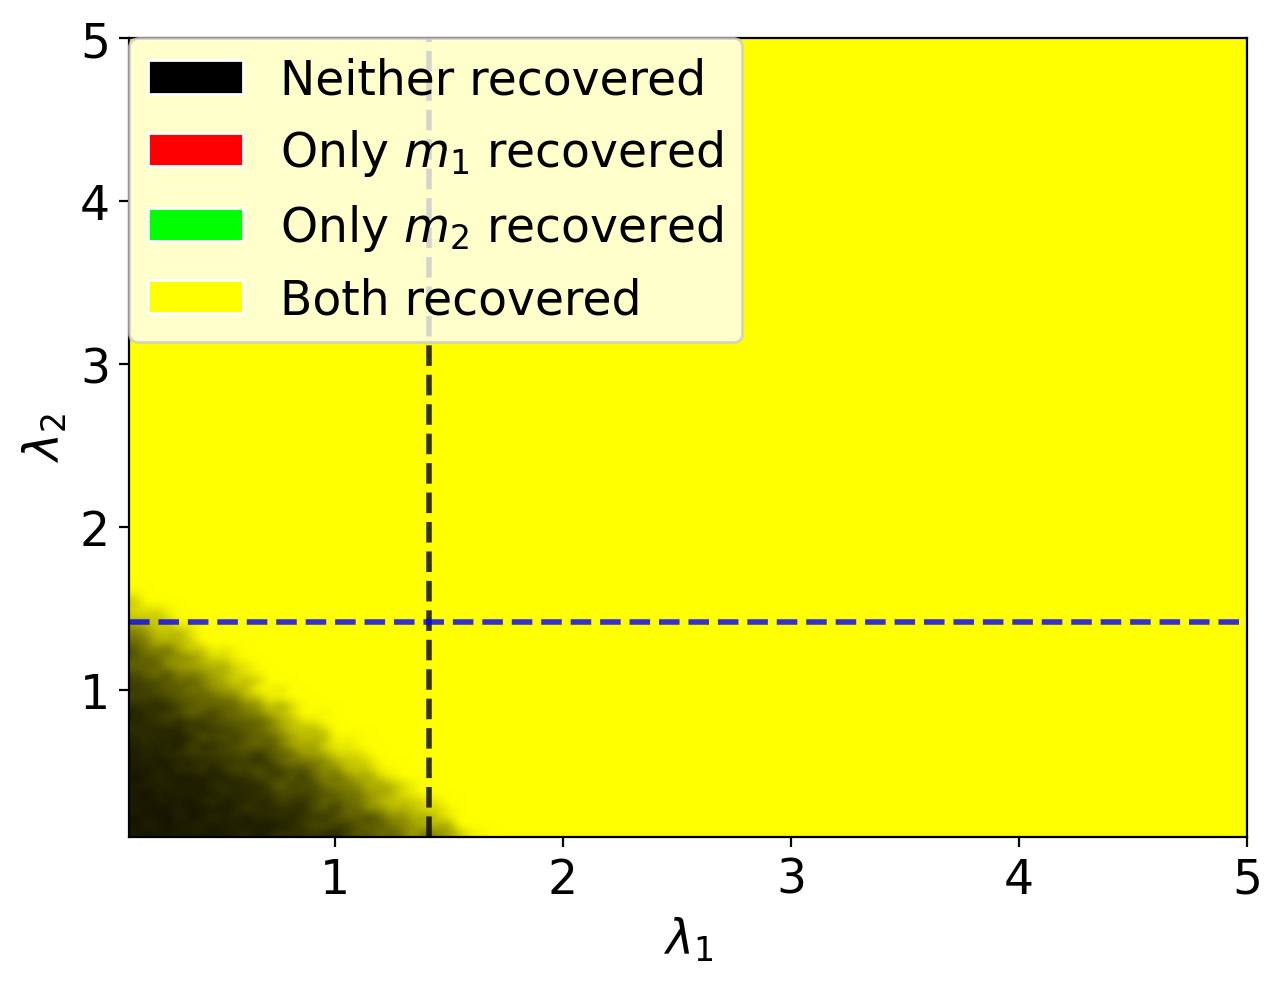
\includegraphics[width=\textwidth]{fig/fig_phase_transition/Phase_Diagram_alpha=0.71_rho=1.00.png}
        \caption{}
    \end{subfigure}
    \centering
    \caption{Phase diagram of the overlap with the estimator as a function of $\lambda_1$ and $\lambda_2$ for a) $\rho=0.0$, b) $\rho = 0.1$, c) $\rho=0.2$, d) $\rho = 0.3$, e) $\rho=0.5$, f) $\rho = 1.0$. With theoretical BBP threshold at $\lambda_1=\lambda_2=\frac{1}{\alpha}=1.41$ in blue and black.}
    \label{fig:Phase_Diagram_1}
\end{figure}
\noindent
Simulation here is run using $n = 300$.
For each pair $(\lambda_1, \lambda_2)$ we record the two recovery overlaps $m_1$ and $m_2$ between the estimator and the planted spikes. To visualise both quantities simultaneously, each pixel of the phase diagram is rendered as an RGB colour whose red and green channels encode the two overlaps independently: $R = m_1 / m_{\max}$ and $G = m_2 / m_{\max}$, clipped to $[0,1]$, with $m_{\max} = 0.5$ chosen as the maximum meaningful per-spike overlap. Four regimes are then directly readable from the resulting image. Black pixels ($R = G = 0$) mark the region where neither spike is recovered. Pure red ($R = 1$, $G = 0$) marks the region where only $m_1$ is recovered, and pure green ($R = 0$, $G = 1$) the region where only $m_2$ is recovered. Yellow pixels ($R = G = 1$), obtained by the additive superposition of red and green, mark the region where both spikes are recovered simultaneously. Smooth gradations between these four corners reflect partial recovery.








\subsection{Using Fisher ~EWC}
\subsubsection{Fisher matrix}
For a model with parameters $\theta$, the Fisher matrix $F$ was previously defined by Eq. \ref{fisher_first_expression} as:
\begin{equation}
    F_{ij} = \mathbb{E}\left[ \frac{\partial \log p(y \mid x, \theta)}{\partial 
    \theta_i} \cdot \frac{\partial \log p(y \mid x, \theta)}{\partial \theta_j} 
    \right],
\end{equation}
One can relate it to the spike model, where $\theta \leftrightarrow \hat{\vect{x}}$ and $\log p(y \mid \cdot, \theta) \leftrightarrow -\mathcal{L}(\vect{x})$ as minimizing the loss is equivalent to maximizing the log likelihood:
\begin{equation}
    \mathcal{F}(\vect{x})=\mathbb{E} [\vect \nabla_x\mathcal{L}(\vect{x})\vect \nabla_x \mathcal{L}(\vect{x})^\top]
\end{equation}
The convergence of $\mathcal{F}_{\mathrm{MS}}(\hat{\vect{x}}^{(1)})$ toward $\mathcal{F}_{\mathrm{MS}}(\vect{x}_1)$ as $\lambda_1$ grows is verified numerically in Appendix~\ref{adix:fisher-conv}.

\paragraph{Fisher matrices of the misspecified and specified losses}
Both Fisher matrices admit closed-form expressions, obtained by carrying out the expectation with the Wigner identity $\mathbb{E}[\vect W \vect A \vect W] = \sigma^2(\mathrm{Tr}(\vect A)\,\vect I + \vect A^\top)$ (Property~\ref{prop:wigner_expectation}). The full step-by-step derivations are deferred to Appendix~\ref{adix:fisher}; we report here only the results.

\noindent
For the misspecified loss $\mathcal{L}(\vect{x}) = -\tfrac{1}{4} \|\vect Y - \vect{x}\vect{x}^\top\|_F^2$, the Fisher matrix reads
\begin{equation}
    \boxed{\mathcal{F}_{\mathrm{MS}}(\vect{x}) = (\lambda-1)^2\vect{x}\vect{x}^\top + \frac{1}{n}(\vect I + \vect{x} \vect{x}^\top)}
    \label{eq:fisher_ms}
\end{equation}
while for the specified loss $\mathcal{L}(\vect{x}) = -\tfrac{1}{4} \|\vect Y - \lambda\vect{x}\vect{x}^\top\|_F^2$, it reduces to
\begin{equation}
    \boxed{\mathcal{F}_{\mathrm{S}}(\vect{x}) = \frac{\lambda^2}{n}(\vect I + \vect{x}\vect{x}^\top )}.
\end{equation}


\subsubsection{Stationarity equation for EWC}

In the previous sections, we introduced the multi-task spiked model together with a quadratic loss that measures the average reconstruction error across tasks. This point of view is naturally adapted to a simultaneous multi-task formulation. However, one of the main motivations behind continual learning is instead \emph{sequential} learning: one first learns a task, then receives a new one, and would like to update the estimator without forgetting the previous task.

This is precisely the philosophy of Elastic Weight Consolidation (EWC). In the present setting, this means the following. One first processes task $1$ and obtains an estimator $\hat x^{(1)}$. Then, when task $2$ is observed, one minimizes a new loss that combines: 
(i) a data-fitting term for task $2$, and 
(ii) a quadratic penalty that discourages the new estimator from moving too far away from $\hat x^{(1)}$ along directions deemed important for task $1$.

The importance of these directions is encoded by a Fisher-type matrix computed after task $1$. In standard EWC, this matrix is then \emph{frozen} during the optimization of task $2$. Therefore, when studying the task-$2$ optimization problem, the Fisher matrix is treated as a fixed matrix, determined by task $1$ and by the estimator obtained at the end of the first stage.

% We now introduce an analogue of Elastic Weight Consolidation (EWC) in the present spiked setting. The main point is that, unlike the previous quadratic losses, the corresponding stationarity equation is generally affine rather than homogeneous. As a consequence, one does not directly obtain a plain top-eigenvector problem. Instead, the natural object is an inverse or resolvent-type formula built from a linear operator and a non-zero source term.

\begin{defn}[First-stage estimator: Single spike estimation]
We first process task $1$ alone. In the simplest version of the construction, we define $\hat x^{(1)}$ as the estimator obtained by minimizing the mis-specified task-$1$ loss
\[
\mathcal{L}_{\mathrm{1,MS}}(\vect x) = -\tfrac{1}{4}\,\|\vect Y_1 - \vect x \vect x^\top\|_F^2 .
\]
Equivalently, up to normalization, scalar shifts, and lower-rank corrections, this leads to the standard spectral estimator based on the top eigenvector of $\vect Y_1$.
\end{defn}

\begin{defn}[Second-stage estimator: EWC-type loss for the spiked model]
Assume that task $1$ has already been processed and has produced an estimator $\hat{\vect x}^{(1)}\in\mathbb R^n$. Let $\vect F_1$ denote either the Fisher matrix or the pseudo-Fisher matrix associated with task $1$.

Given a loss $\mathcal L_2(\vect x)$ associated with task $2$, we define the EWC-type regularized loss by
\begin{equation}
    \mathcal L_{\mathrm{EWC}}(\vect x)
    :=
    \mathcal L_2(\vect x)
    +
    \mu_R (\vect x-\hat{\vect x}^{(1)})^\top \vect F_1 (\vect x-\hat{\vect x}^{(1)})
    \label{eq:LossEWC}
\end{equation}

where $\mu_R\geq 0$ is a regularization parameter.
\end{defn}

\begin{rem}
The standard quadratic EWC penalty is
\[
(\vect x-\hat{\vect x}^{(1)})^\top \vect F_1 (\vect x-\hat{\vect x}^{(1)})
=
\|\vect F_1^{1/2}(\vect x-\hat{\vect x}^{(1)})\|_2^2
\]
Writing instead $\|\vect F_1(\vect x-\hat{\vect  x}^{(1)})\|_2^2$ would lead to the matrix $\vect F_1^2$ in the quadratic form, which is a different regularization.
\end{rem}

\begin{defn}[Resolvent of a matrix $\vect A$]
    Given a matrix $\vect A$, the resolvent may be defined as:
    \begin{equation}
        \vect R(z; \vect A) = (\vect A - z\vect I)^{-1}
        \label{resolvent}
    \end{equation}
    for which $(\vect A - z\vect I)$ is invertible. We will write $\vect R(z; \vect A)$ as $\vect R_{\vect A}(z)$ or even $\vect R(z)$.
    \label{def:resolvent}
\end{defn}


\subsection{Methods inspired by EWC}
Following the EWC philosophy, we combine the misspecified task-$2$ loss with the Fisher penalty anchored at the first-stage estimator $\hat{\vect x}^{(1)}$:
\[
    \mathcal L_{\mathrm{EWC}}(\vect{x}) = \mathcal{L}_{\mathrm{2,MS}}(\vect{x}) + \mu_R (\vect{x} - \hat{\vect{x}}^{(1)})^\top \vect F_1(\vect{x} - \hat{\vect{x}}^{(1)}),
\]
with $\hat{\vect{x}}^{(1)}$ the optimizer of the task-$1$ misspecified loss on the first spike only. Computing the gradient and imposing the stationarity condition $\vect \nabla \mathcal L_{\mathrm{EWC}}(\vect{x})=0$ together with the constraint $\norm{\vect x}^2=1$ yields, after linearization, an affine system in $\vect x$ (the full derivation is given in Appendix~\ref{adix:ewc}):
\begin{equation}
    \boxed{\vect A \vect{x} = \vect b}, \qquad
    \vect A = \vect Y_2 -\vect I + 2\mu_R \vect F_1, \qquad
    \vect b = 2\mu_R \vect F_1\vect{\hat x}^{(1)}.
    \label{eq:stationary_condition}
\end{equation}
The associated Hessian is $\mathcal{H_{\text{EWC}}} = \rdmmat Y_2 - \vect I  + 2 \mu_R \rdmmat F_1$.


\noindent
Defining $\vect M :=\vect Y_2 + 2\mu_R \vect F_1$, a matrix collecting the data and the EWC penalty together, we have $\vect A =\vect M - \vect I$. Whenever $\vect A$ is invertible, the system solves explicitly into the final estimator
\begin{equation}
    \boxed{
    \hat{\vect{x}}^{(2)} = 2\mu_R \vect R_{\vect A}(1)\vect F_1 \vect{\hat x}^{(1)}}
    \label{eq:final_estimator}
\end{equation}
with $\vect R_{\vect A}(1) = (\vect M - \vect I) ^{-1}$ the resolvent of $\vect M$ evaluated at $z = 1$ according to Def.~\ref{def:resolvent}.


\subsubsection{Methods to recover signal}
We introduce two different methods to recover the signal.

\begin{defn}[Method A -- spectral approach]
Neglecting the inhomogeneous term $\vect{b}$, we estimate the signal via
the leading eigenvector of the Hessian:
\[
    \hat{\vect{x}}^{(2)}_A
    = \operatorname{top-eigenvector}(\mathcal{H}_{\mathrm{EWC}}),
    \qquad
    \mathcal{H}_{\mathrm{EWC}}
    = \vect{Y}_2 - \vect{I} + 2\mu_R\vect{F}_1.
\]
This eigenvector is unit-normalised by construction.
\end{defn}


\begin{defn}[Method B -- resolvent approach]
Assuming $\vect{A}$ is invertible, the estimator is computed directly from
the linear system~\eqref{eq:stationary_condition}:
\[
    \hat{\vect{x}}^{(2)}_B
    = 2\mu_R\,\vect{A}^{-1}\vect{F}_1\,\hat{\vect{x}}^{(1)}.
\]
\end{defn}

\begin{rem}[Norm constraint and Lagrange regularisation]
In practice, $\mathcal{H}_{\mathrm{EWC}}$ has near-zero eigenvalues
(its determinant is of order $10^{-52}$, see Figure~\ref{fig:Fisher_Hess}),
so $\vect{A}$ is numerically singular and Method~B cannot be applied
directly.

To enforce the hard constraint $\|\vect{x}\|=1$, we introduce the
Lagrangian
\[
    J(\vect{x},\lambda)
    = \mathcal{L}_{\mathrm{EWC}}(\vect{x})
    + \lambda\,g(\vect{x}), \qquad
    g(\vect{x}) = \|\vect{x}\|^2 - 1.
\]
The two stationarity conditions are:
\begin{align}
    \partial_\lambda J(\vect{x},\lambda) = 0
        &\;\Longrightarrow\; g(\vect{x}) = 0,
        \quad\text{i.e.}\quad \|\vect{x}\|^2 = 1, \\
    \nabla_{\!\vect{x}} J(\vect{x},\lambda) = 0
        &\;\Longrightarrow\;
        \bigl(\vect{M} - (1+\lambda)\vect{I}\bigr)\vect{x} = \vect{b}.
\end{align}
The second equation shows that the Lagrange multiplier $\lambda$ acts as a
\emph{spectral shift}: it moves the evaluation point of the resolvent from
$z=1$ to $z = 1+\lambda$, regularising the inversion.  The constrained
estimator is therefore
\begin{equation}
    \boxed{
      \hat{\vect{x}}^{(2)}
      = 2\mu_R\,\vect{R}_{\vect{M}}(1+\lambda)\,
        \vect{F}_1\,\hat{\vect{x}}^{(1)}
    }
    \label{eq:final_estimator_lagrange}
\end{equation}
where $\vect{R}_{\vect{M}}(z) = (\vect{M} - z\vect{I})^{-1}$, and
$\lambda$ is the unique scalar satisfying the norm equation
\begin{equation}
    g(\lambda) \;:=\; \bigl\|\hat{\vect{x}}^{(2)}(\lambda)\bigr\|^2 - 1 = 0.
    \label{eq:norm_constraint}
\end{equation}





\subsubsection{Numerics}
\paragraph{Selection of the regularization parameter}
The regularization parameter  $\mu$ needs to be such that the estimator can learn the second task $\vect x_2$ without forgetting the first one $\vect x_1$. Ideally, the best regularization parameter is found minimizing the loss, as shown on Fig. \ref{fig:Phase_Diagram_1} (a), but we observed that the $\mu$ found using this method wasn't always the one optimizing the overlap as well as we could hope, so we instead turned to another choise of this regularization parameter: the one that maximizes the overlap, as shown on Fig. \ref{fig:Phase_Diagram_1} (b).

\begin{figure}[H]
    \begin{subfigure}{0.52\textwidth}
        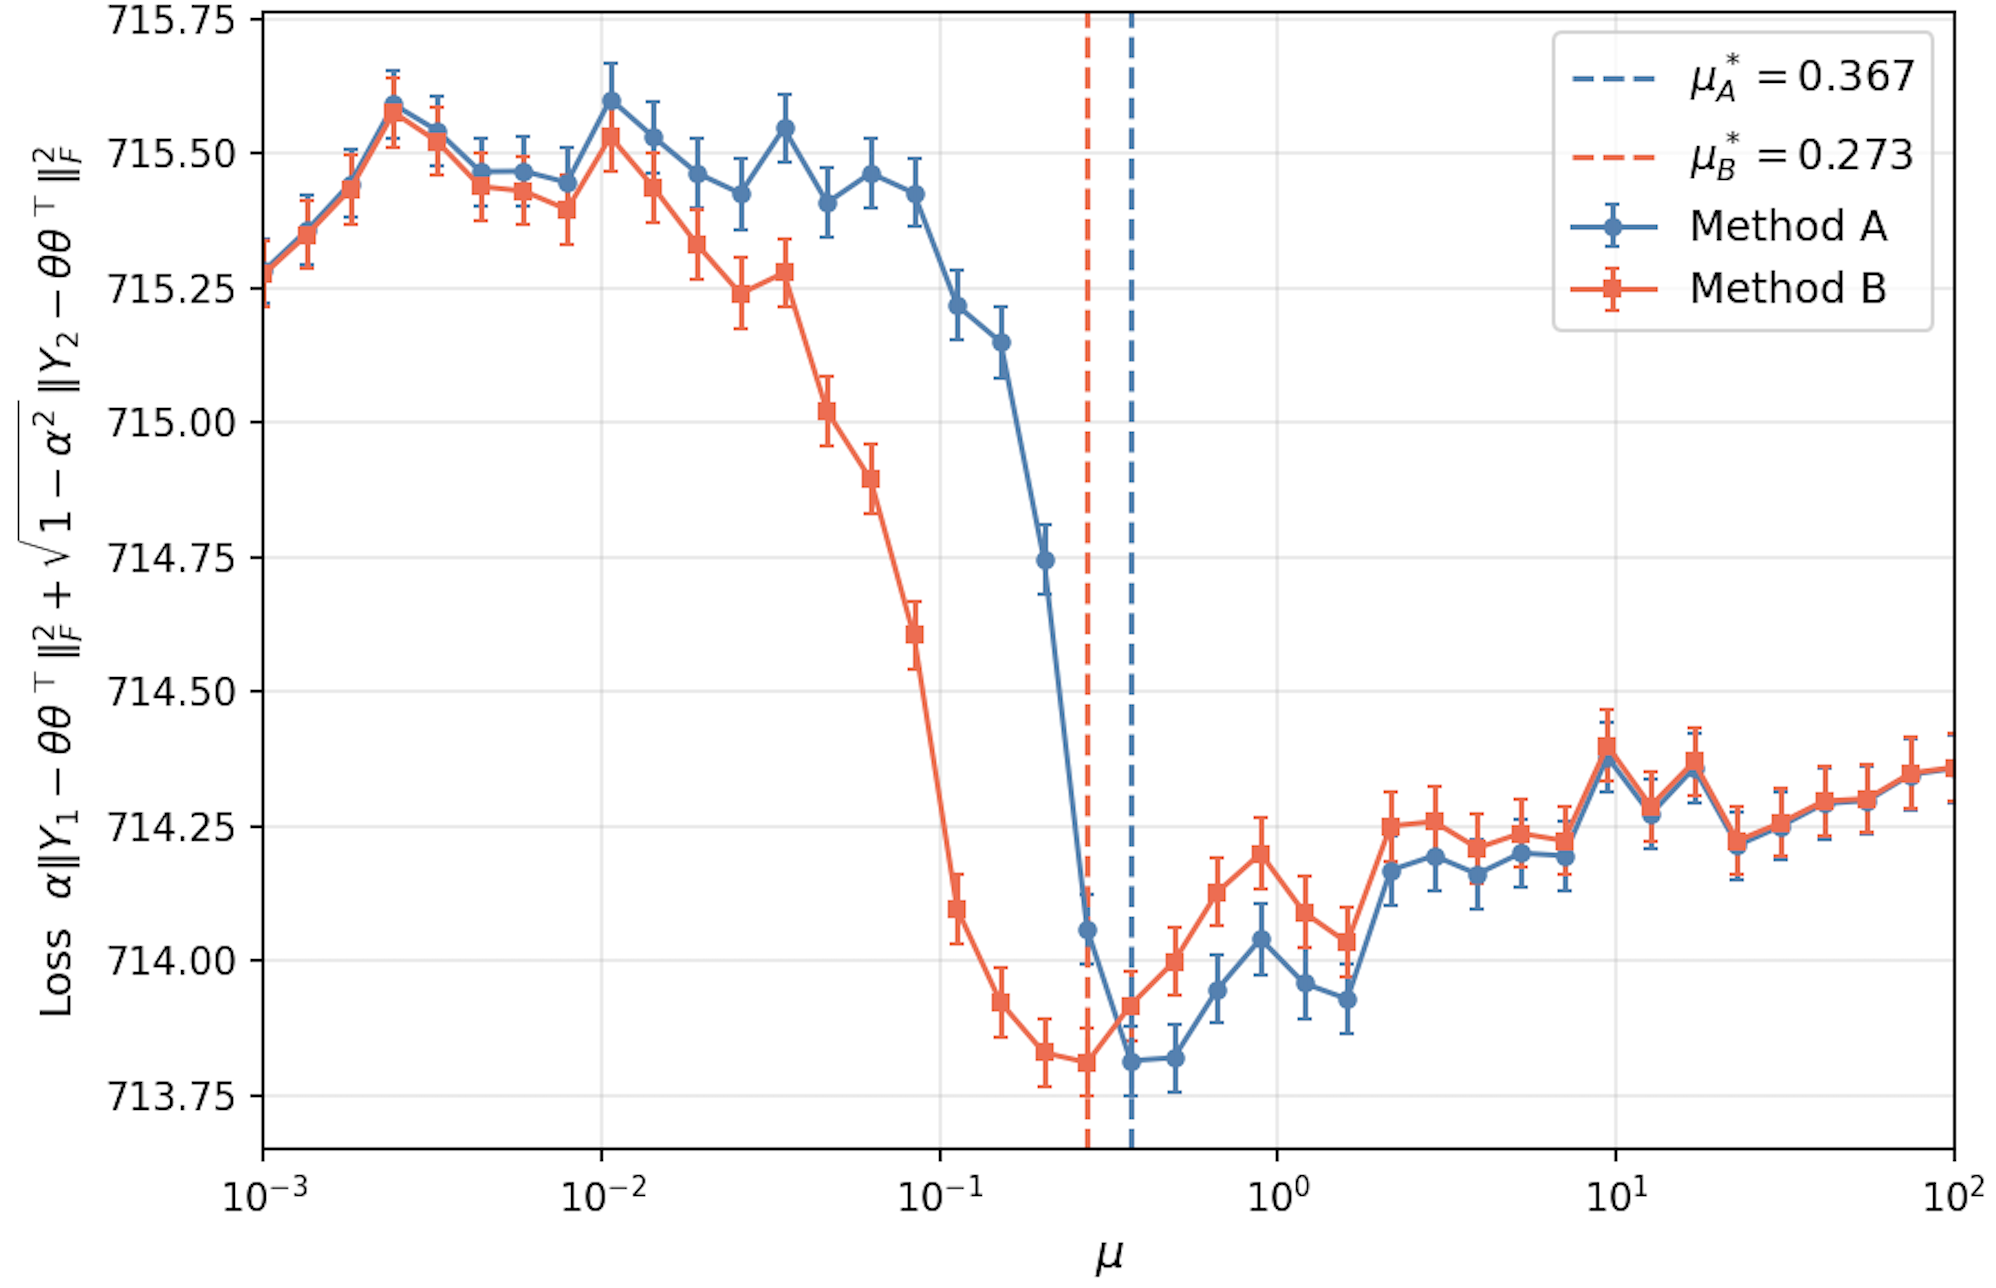
\includegraphics[width=\textwidth]{fig/cluster/loss_vs_mu.png}
                \caption{}
    \end{subfigure}
    \begin{subfigure}{0.44\textwidth}
        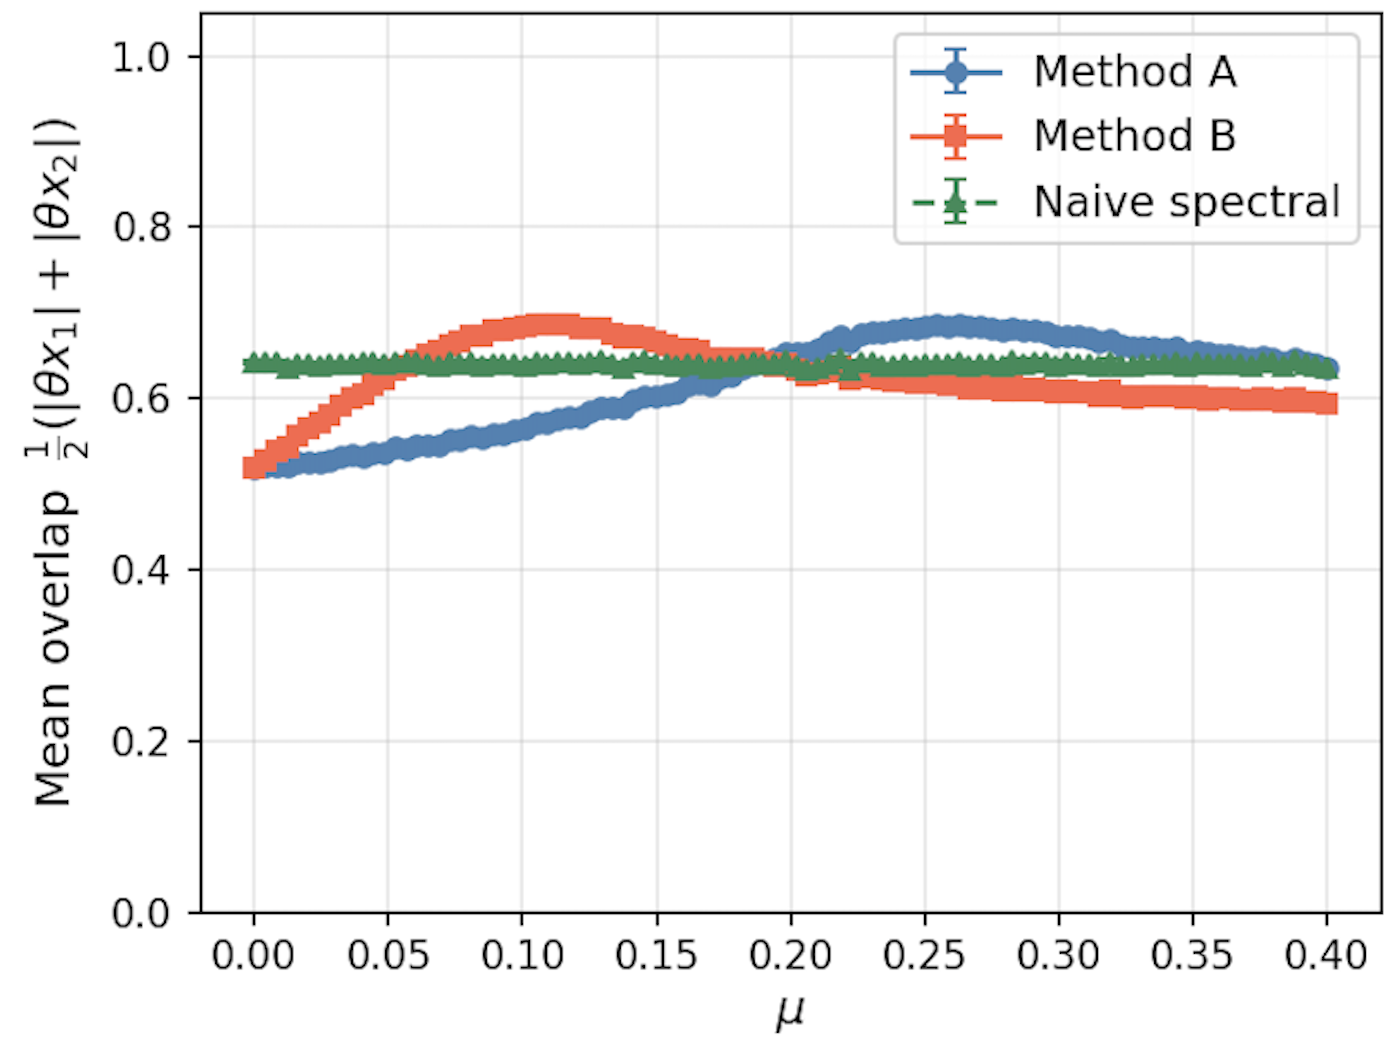
\includegraphics[width=\textwidth]{fig/cluster/AB_vs_mu_rho_0.20.png}
                \caption{}
    \end{subfigure}
   
    \caption{\centering Evaluation of the Loss (a) and the mean overlap over the two signals (b) as a function of the regularization parameter $\mu$.}
    \label{fig:Phase_Diagram_1}
\end{figure}
For Fig. \ref{fig:Phase_Diagram_1} (a), each value plotted is the mean value of the loss across 1000 simulations. In practice, we won't go that far, which will increase the variance in the loss, and therefore the result of the $\mu$ chosen. In both cases, an optimal $\mu$ appears. For stability reasons, the selection of $\mu$ is done by finding $\mu$ such that it maximizes the mean overlap (see annex \ref{adix:overlap_loss}).

\subsection{Evaluation of the methods}
We evaluated the recovery performance of methods A and B against the naïve method previously used. For each of the two following plots, we each time varied $\rho$ and $\lambda_1$ along 50 values, for each of those values, we ran 400 simulations to find the best $\mu$ (the one maximizing the mean overlap), and plotted the desired result. For the naive method, the importance factor $\alpha$ is chosen so that both signals have the same importance ($\alpha=\sqrt{0.5}$). When the parameter choice is such that $\rho=0.2$, $\lambda_1 = 3$ and $\lambda_2 = 2$ (when the parameter in question is not varied). The results are shown in Fig. \ref{fig:comparaison_rho} and Fig. \ref{fig:comparaison_l1}. 

\begin{figure}[H]
    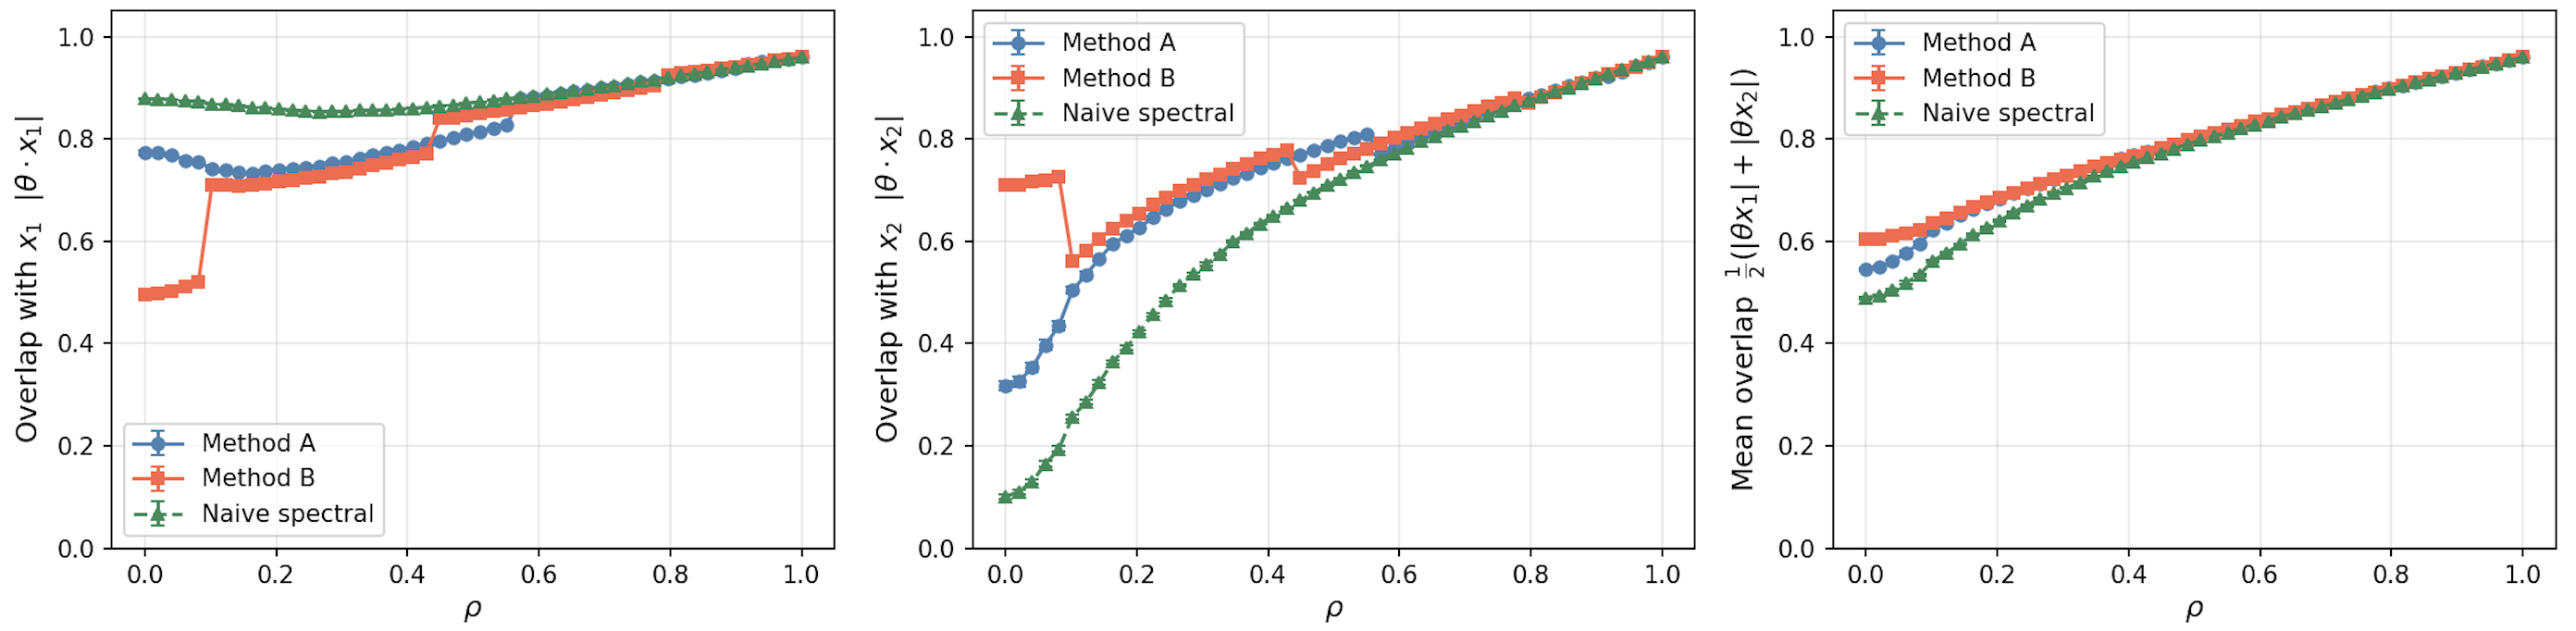
\includegraphics[width=\textwidth]{fig/cluster/overlaps_vs_rho.png}
    
    \caption{\centering Overlap with signal 1, signal 2, and mean overlap  as a function of correlation $\rho$ for the three methods (naive, A, B).}
    \label{fig:comparaison_rho}
\end{figure}

\begin{figure}[H]
    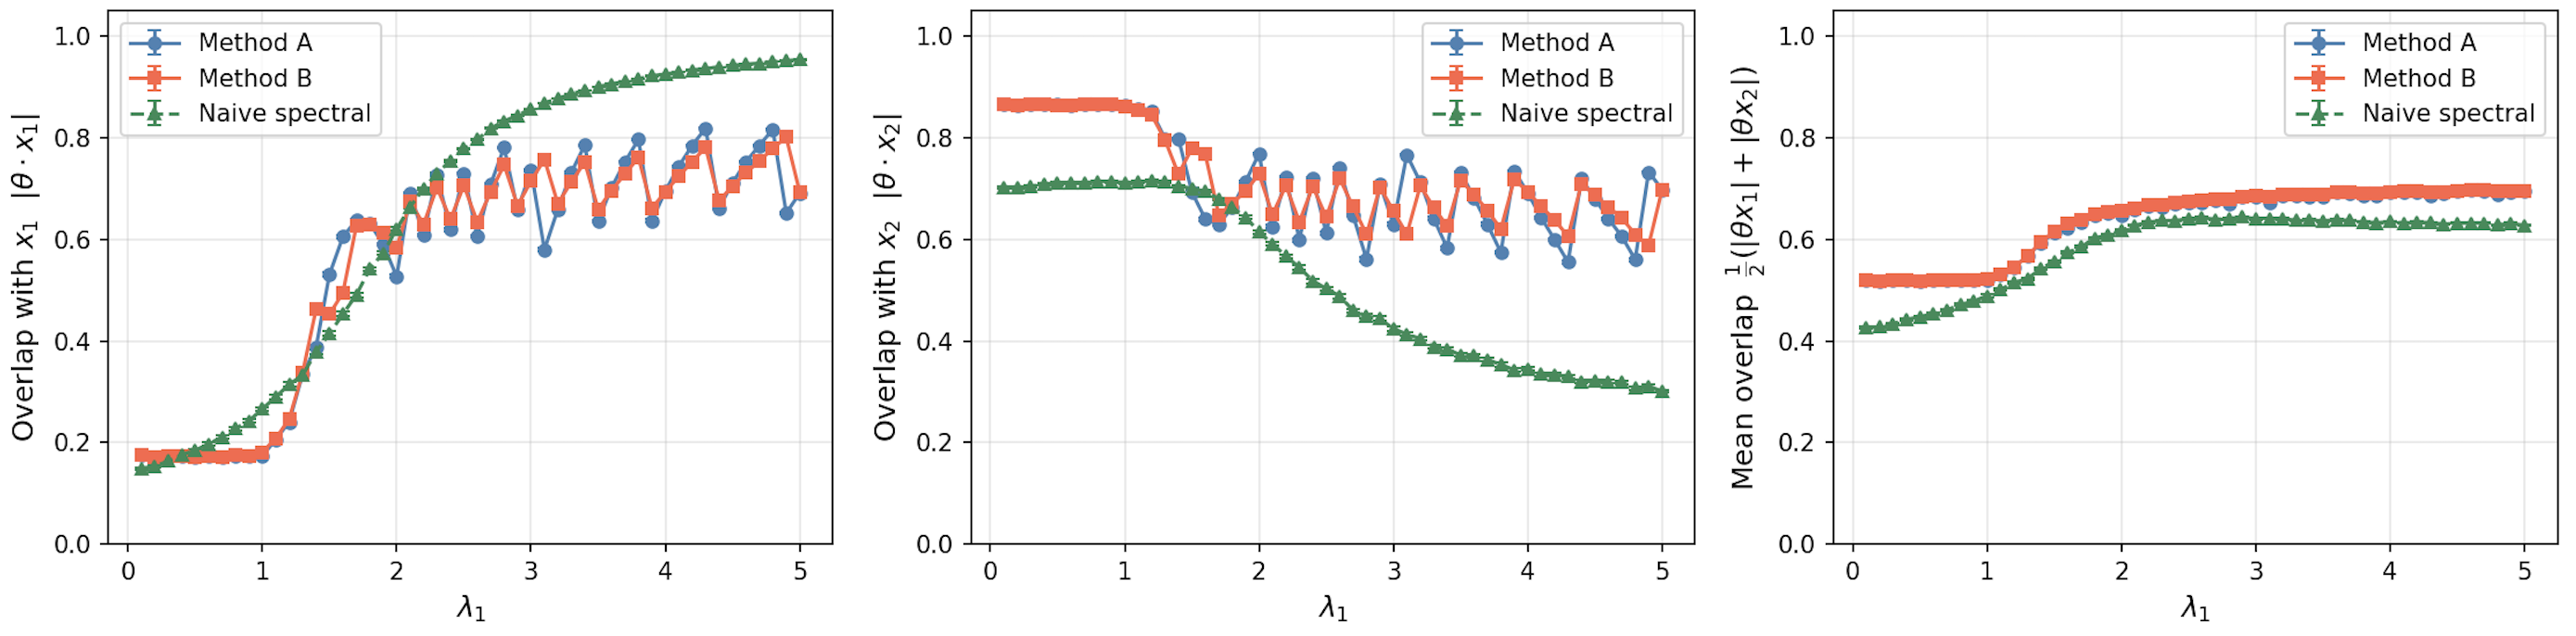
\includegraphics[width=\textwidth]{fig/cluster/overlaps_vs_lambda1.png}
    
    \caption{\centering Overlap with signal 1, signal 2, and mean overlap as a function of $\lambda_1$ for the three methods (naive, A, B).}
    \label{fig:comparaison_l1}
\end{figure}

\paragraph{Discussion}
Figures \ref{fig:comparaison_rho} and \ref{fig:comparaison_l1} show that Methods A and B generally outperform the naive approach. As the correlation parameter $\rho$ increases, the performances of the three methods become closer, indicating that highly correlated signals are easier to recover regardless of the method used. However, for low values of $\rho$, the regularized approaches achieve higher overlap scores and better support recovery. Furthermore, the results obtained by varying $\lambda_1$ highlight the greater robustness of Methods A and B, whose mean overlap remains relatively stable over a wide range of parameter values. In contrast, the naive method is more sensitive to parameter changes. Overall, these results suggest that incorporating regularization improves the exploitation of shared information between signals and leads to more accurate support recovery.

\section{Conclusion}

In this project, we investigated continual learning through the framework of Elastic Weight Consolidation (EWC), combining empirical experiments on neural networks with a theoretical analysis based on spiked random matrix models. We first reproduced the main phenomena reported in the original EWC literature on the permuted-MNIST benchmark, highlighting the ability of Fisher-based regularization to mitigate catastrophic forgetting while preserving the capacity to learn new tasks.

To gain theoretical insight into these mechanisms, we introduced a multi-task extension of the spiked Wigner model, where several correlated signals must be recovered from noisy observations. This simplified framework allowed us to study the role of task correlations, signal strengths, and spectral phase transitions in a controlled setting. Numerical experiments showed how correlations between tasks can significantly improve recovery performance, even when one of the signals lies below the classical BBP threshold.

Inspired by the EWC philosophy, we derived Fisher-based regularized estimators and proposed two spectral methods. Their performances were compared with a naive multi-task spectral approach. The results demonstrated that incorporating Fisher information leads to more robust estimators, particularly in regimes of low correlation or heterogeneous signal strengths. In these challenging settings, the regularized methods achieved higher overlaps and more stable recovery performances than the naive approach.

Overall, this work illustrates how ideas originating from continual learning can be translated into analytically tractable inference problems. Beyond providing a theoretical interpretation of EWC-like mechanisms, the proposed framework opens several directions for future research, including a rigorous asymptotic analysis of the proposed estimators, the study of Approximate Message Passing algorithms in the multi-task setting, and the characterization of the corresponding phase transitions and optimal recovery thresholds.
% \begin{rem}[Why EWC does not directly give a plain spectral method]
% For a standard spectral method, one typically looks for an eigenvector of a linear operator. By contrast, the EWC stationarity condition takes the form
% \[
% A_\tau u=b,
% \]
% with a non-zero right-hand side $b$. Therefore, the estimator is not obtained by solving a homogeneous eigenvalue problem, but rather by applying an inverse operator to a source term. The homogeneous part still defines a natural spectral operator, but the full EWC estimator is more faithfully described by a resolvent-type formula.
% \end{rem}


% \begin{exo}[EWC Loss for spiked models]\leavevmode\\
% Try to write the equivalent of the EWC loss for the spiked models.
% \end{exo}
% Hugo: This I will give and also the spectral method, they will redo the calculation from the loss to the spectral methods. 

% Then, we will get a spectral method out of it. 




\bibliographystyle{unsrt}
\bibliography{bib}

\appendix
\section{Appendix}

\subsection{EWC experimental settings (permuted MNIST)}\label{adix:EWC_1}
The continual-learning experiment of Section~\ref{sec:ewc} follows the permuted-MNIST protocol of Kirkpatrick et al.~\cite{Kirkpatrick_2017}. A set of tasks (\emph{A}, \emph{B}, \emph{C}) is built from the MNIST dataset~\cite{LeCun1998}: for each task a fixed random permutation of the input pixels is drawn and applied to all images, so that every task is of equal difficulty to the original problem but requires a different solution. A single multi-layer perceptron is then trained sequentially on the three tasks, and the same architecture is re-used for the three compared methods: plain SGD, $L_2$ regularization toward the previous parameters, and EWC. After training on each task, the diagonal Fisher information is estimated empirically by averaging the squared per-parameter gradients of the log-likelihood over a batch of samples from that task, evaluated at the parameters obtained at the end of the task; the Fisher contributions of successive tasks are summed. Test accuracy is monitored on all three tasks throughout the whole training timeline, producing the curves of Figure~\ref{fig:EWC_1}.

\subsection{Consistency between normalizations}\label{adix:norm}
Substituting $  \rdmmat W = \sqrt{n}\rdmmat Z$ into Definition~\ref{def:spiked-wigner} and dividing by $\sqrt{n}$, we get:
    \[
    \frac{\widetilde{\rdmmat Y}}{\sqrt{n}} = \frac{\lambda}{n}\vect u \vect u ^T + \rdmmat Z
    \]
    we now take $\vect x = \frac{\vect u}{\norm{\vect u}}$ so that $\norm{\vect x} = 1$, we have:
    \[
    \frac{\widetilde{\rdmmat Y}}{\sqrt{n}} = \frac{\lambda}{n}\vect x \vect x ^T \norm{u}^2 + \rdmmat Z
    \]
    finally, taking the ($n \rightarrow \infty$) limit and using that $\frac{\norm{\vect u }^2}{n}\rightarrow1$ by assumption, in this limit:
    \[
    \frac{\widetilde{\rdmmat Y}}{\sqrt{n}} = \lambda\vect x \vect x ^T + \rdmmat Z = \rdmmat Y
    \]
\noindent
This yields the other normalization
\[
    \rdmmat Y = \lambda \,\vect x \vect x^T + \rdmmat Z,
\]
used throughout the report (Eq.~\eqref{norm2}), where $\|\vect x\|=1$ and $\rdmmat Z = \frac{1}{\sqrt n}\rdmmat W$ is equivalent to Definition~\ref{def:spiked-wigner}. In particular, both have the same asymptotic spectral behaviour, as the eigenvalues of $\rdmmat Y$ and $\widetilde{\rdmmat Y}$ are the same up to a $\frac{1}{\sqrt{n}}$ factor.

\subsection{Gradient and Hessian of the single-spike misspecified loss}\label{adix:spectral-grad}
Differentiating the misspecified loss~\eqref{eq:MSloss} component-wise gives
\begin{equation}
    \partial_{\hat{x}_i} \mathcal{L} = -\frac{1}{2} \partial_{\hat{x}_i}\sum_{k,l} (Y_{k,l} - \hat{x}_k \hat{x}_l)^2 = \sum_{l}  (Y_{i,l} - \hat{x}_i \hat{x}_l)\hat{x}_l ,
\end{equation}
which in vector form reads
\begin{equation}
    \vect{\nabla_{\hat{\vect{x}}}}\mathcal{L} = \rdmmat Y \hat{\vect{x}} - \norm{\hat{\vect{x}}}^2 \hat{\vect{x}},
\end{equation}
as stated in the main text. The Hessian then follows as $\mathcal{H} = \vect{\nabla}_{\hat{\vect{x}}} [(\rdmmat Y  -\rdmmat I) \hat{\vect{x}}] = \rdmmat Y  -\rdmmat I$ once the normalization $\norm{x}=1$ is used.

\subsection{Gradient and Hessian of the naive multi-task loss}\label{adix:naive-grad}
Differentiating the multi-task MS loss $\mathcal{L}_{\mathrm{MSE}}$ term by term, each Frobenius term contributes as in the single-spike case, giving the gradient
\begin{equation}
    \vect{ \nabla} \mathcal{L}_{\mathrm{MSE}}(\vect x) = \alpha (\rdmmat Y_1 - \rdmmat I)\vect x + \sqrt{1-\alpha^2} (\rdmmat Y_2 - \rdmmat I)\vect x .
\end{equation}
Differentiating once more yields the Hessian
\begin{equation}
    \mathcal{H} = \alpha \rdmmat Y_1 + \sqrt{1-\alpha^2} \rdmmat Y_2 - \rdmmat I ( \alpha + \sqrt{1-\alpha^2}) = \rdmmat Y - \rdmmat I ( \alpha + \sqrt{1-\alpha^2}),
\end{equation}
where $\rdmmat Y := \alpha \rdmmat Y_1 + \sqrt{1-\alpha^2}\,\rdmmat Y_2$ is the observation of Eq.~\eqref{eq:2spikes}.

\subsection{Derivation of the Fisher matrices}\label{adix:fisher}

\paragraph{Fisher matrix of misspecified loss}

One can use the expression of the misspecified loss :
\[
    \mathcal{L}(\vect{x}) = -\tfrac{1}{4} \|\vect Y - \vect{x}\vect{x}^\top\|_F^2
\]
and compute:
\[
    \vect \nabla_x \mathcal{L}(\vect{x}) = (\vect Y - \vect{x} \vect{x}^\top) \vect{x} = \vect Z\vect{x}
\]
with $\vect Z := \vect Y - \vect{x} \vect{x}^\top$, to get:
\[
    \vect \nabla_x \mathcal{L}(\vect{x}) \vect \nabla_x \mathcal{L}(\vect{x})^\top = \vect Z \vect{x} \vect{x}^\top \vect Z^\top = \vect Z \vect{x}\vect{x}^\top \vect Z
\]
as $(\vect Z^\top = \vect Z)$. \\
The misspecified Fisher matrix can be re-written:
\[
    \mathcal{F}_{\mathrm{MS}}(\vect{x}) = \mathbb{E}[\vect Z \vect{x}\vect{x}^\top \vect Z]
\]
with
\[
    \vect Z = \vect Y - \vect{x} \vect{x}^\top = (\lambda - 1) \vect{x} \vect{x}^\top + \vect W
\]
where $\vect W$ is simply the bulk of the noise, a symmetric Gaussian Wigner matrix.\
Developing the result yields:
\[
\mathbb{E} [\vect Z \vect{x} \vect{x}^\top \vect Z] = (\lambda - 1)^2 \vect{x} \vect{x}^\top + \mathbb{E}[\vect W \vect{x} \vect{x}^\top \vect W]
\]
as $\mathbb{E}[W_{ij}]=0$ and $\mathbb{E}[W_{ij}^2]=\sigma^2=\frac{1}{n}$.
\begin{property} \label{prop:wigner_expectation}
\[
    \mathbb{E}[\vect W \vect A \vect W] = \sigma^2(\mathrm{Tr}(\vect A) \vect I + \vect A^\top).
    \label{proof_tali_1}
\]
\end{property}

\noindent
One can also use Prop. \ref{prop:wigner_expectation}:
\[
    \mathbb{E}[\vect W \vect A \vect W] = \sigma^2(\mathrm{Tr}(\vect A) \vect I + \vect A^\top) = \frac{1}{n}(\mathrm{Tr}(\vect A) \vect I + \vect A^\top)
\]
\noindent
Applying this to $\vect A = \vect{x} \vect{x}^\top$ with $\|\vect{x}\| = 1$ and $\sigma = \frac{1}{\sqrt{n}}$ gives
$\mathrm{Tr}(\vect A) = 1$ and $\vect A^\top = \vect A$
\[
\mathbb{E}[\vect W \vect{x} \vect{x}^\top \vect W] = \frac{1}{n}(\vect I + \vect{x} \vect{x}^\top)
\]
reinserting in the previous expression,
\[
\mathbb{E}[\vect Z \vect{x}\vect{x}^\top \vect Z] = (\lambda-1)^2 \vect{x}\vect{x}^\top + \frac{1}{n}(\vect I + \vect{x} \vect{x}^\top)
\]
gives the final expression of the Fisher matrix:
\begin{equation}
    \mathcal{F}_{\mathrm{MS}}(\vect{x}) = (\lambda-1)^2\vect{x}\vect{x}^\top + \frac{1}{n}(\vect I + \vect{x} \vect{x}^\top)
\end{equation}

\paragraph{Fisher matrix of specified loss}
Using the expression of the specified loss :
\[
    \mathcal{L}(\vect{x}) = -\tfrac{1}{4} \|\vect Y - \lambda\vect{x}\vect{x}^\top\|_F^2
\]
One can compute:
\[
    \vect \nabla_x \mathcal{L}(\vect{x}) = \lambda(\vect Y - \lambda \vect{x} \vect{x}^\top) \vect{x} = \lambda \vect Z \vect{x}
\]
with $\vect Z := \vect Y - \lambda\vect{x} \vect{x}^\top$ as before, to get:
\[
    \vect \nabla_x \mathcal{L}(\vect{x}) \vect \nabla_x \mathcal{L}(\vect{x})^\top = \lambda^2\vect Z \vect{x} \vect{x}^\top \vect Z^\top = \lambda^2\vect Z \vect{x}\vect{x}^\top \vect Z
\]
as $(\vect Z^\top = \vect Z)$. \\
The specified Fisher matrix can be re-written:
\[
    \mathcal{F}_{\mathrm{S}}(\vect{x}) = \lambda^2\mathbb{E}[\vect Z \vect{x}\vect{x}^\top \vect Z]
\]
with
\[
    \vect Z =\vect Y - \lambda\vect{x} \vect{x}^\top = \lambda \vect{x} \vect{x}^\top + \vect W  - \lambda \vect{x} \vect{x}^\top= \vect W
\]
where $\vect W$ is simply the bulk of the noise, a symmetric Gaussian Wigner matrix.\
So:
\[
\mathbb{E} [\vect Z \vect{x} \vect{x}^\top \vect Z] = \mathbb{E}[\vect W \vect{x} \vect{x}^\top \vect W]
\]
One can also use Prop. \ref{prop:wigner_expectation}:
\[
    \mathbb{E}[\vect W \vect A \vect W] = \sigma^2(\mathrm{Tr}(\vect A) \vect I + \vect A^\top) = \frac{1}{n}(\mathrm{Tr}(\vect A) \vect I +\vect A^\top)
\]
\noindent
Applying this to $\vect A = \vect{x} \vect{x}^\top$ with $\|\vect{x}\| = 1$ and $\sigma = \frac{1}{\sqrt{n}}$ gives
$\mathrm{Tr}(\vect A) = 1$ and $\vect A^\top = \vect A$
\[
\mathbb{E}[\vect W \vect{x} \vect{x}^\top \vect W] = \frac{1}{n}(\vect I +\vect{x} \vect{x}^\top)
\]
reinserting in the previous expression,
\[
\mathbb{E}[\vect Z \vect{x}\vect{x}^\top \vect Z] = \frac{1}{n}(\vect I + \vect{x} \vect{x}^\top)
\]
gives the final expression of the Fisher matrix:
\begin{equation}
    \mathcal{F}_{\mathrm{S}}(\vect{x}) = \frac{\lambda^2}{n}(\vect I + \vect{x}\vect{x}^\top )
\end{equation}
\subsection{Convergence of the Fisher matrix: true signal vs.\ first-stage estimator}
\label{adix:fisher-conv}

In practice, the Fisher matrix $\vect{F}_1$ used in the EWC penalty is evaluated at the first-stage estimator $\hat{\vect{x}}^{(1)}$ rather than at the unknown true signal $\vect{x}_1$. Figure~\ref{fig:fisher_conv} shows that the relative difference between $\mathcal{F}_{\mathrm{MS}}(\vect{x}_1)$ and $\mathcal{F}_{\mathrm{MS}}(\hat{\vect{x}}^{(1)})$ (computed using the theoretical expression of Eq.~\eqref{eq:fisher_ms}) decreases as $\lambda_1$ increases, confirming that the substitution is asymptotically valid in the high-SNR regime. The decay does not depend on $n$ (for $n=1000$), indicating that the convergence is driven by the alignment between $\hat{\vect{x}}^{(1)}$ and $\vect{x}_1$ rather than by the matrix dimension.

\begin{figure}[H]
    \centering
    \begin{subfigure}{0.49\textwidth}
        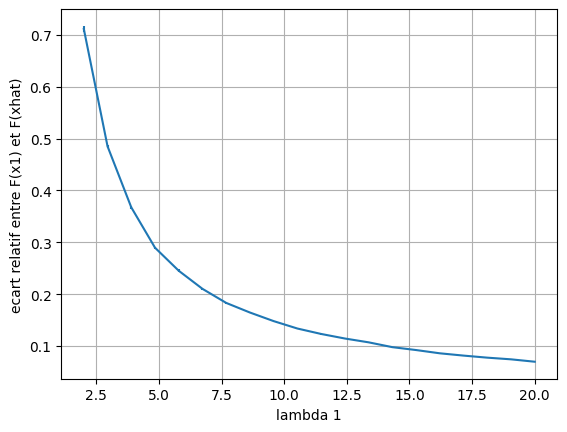
\includegraphics[width=\textwidth]{fig/fisher/ecart_Fisher_x_xhat.png}
        \caption{Linear scale. $n = 1000$.}
    \end{subfigure}
    \begin{subfigure}{0.49\textwidth}
        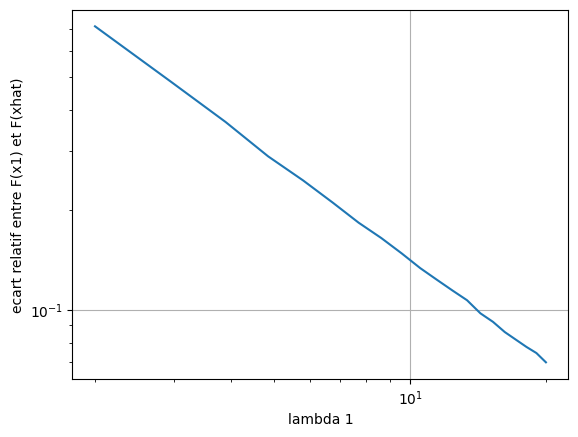
\includegraphics[width=\textwidth]{fig/fisher/ecart_Fisher_x_xhat_loglog.png}
        \caption{Log-log scale. $n = 1000$.}
    \end{subfigure}
    \caption{Relative difference between the Fisher matrix evaluated at the true signal $\vect{x}_1$ and at the first-stage estimator $\hat{\vect{x}}^{(1)}$, as a function of $\lambda_1$. The theoretical Fisher matrix of Eq.~\eqref{eq:fisher_ms} is used throughout.}
    \label{fig:fisher_conv}
\end{figure}


\subsection{Derivation of the EWC spectral estimator}\label{adix:ewc}
One can use the expression of the misspecified loss :
\[
    \mathcal{L}_{\mathrm{i, MS}}(\vect{x}) = -\tfrac{1}{4} \|\vect Y_i - \vect{x}\vect{x}^\top\|_F^2
\]
One can compute:
\[
    \vect \nabla \mathcal{L}_{\mathrm{i,MS}}(\vect{x}) = (\vect Y_i - \vect{x}\vect{x}^\top) \vect{x}
\]
The EWC loss is
\[
    \mathcal L_{\mathrm{EWC}}(\vect{x}) = \mathcal{L}_{\mathrm{2,MS}}(\vect{x}) + \mathcal{L}_{\mathrm{FISHER}}(\vect{x})
\]
with
\[
    \mathcal{L}_{\mathrm{FISHER}}(\vect{x}) =
    \mu_R (\vect{x} - \hat{\vect{x}}^{(1)})^\top \vect F_1(\vect{x} - \hat{\vect{x}}^{(1)}).
\]
with $\hat{\vect{x}}^{(1)}$ the optimizer of $\mathcal{L}_{\mathrm{1,MS}}(\vect{x})$ on the first spike only.\\
Then using $ \vect F^\top=\vect F$ gives
\[
    \vect \nabla [(\vect{x}-\vect{\hat x}^{(1)})^\top \vect F_1 (\vect{x}-\vect{\hat x}^{(1)})]
     =
    2 \vect F_1(\vect{x} - \vect{\hat x}^{(1)}).
\]
Summing the two contributions:
\[
    \vect \nabla \mathcal L_{\mathrm{EWC}}(\vect{x})= (\vect Y_2 - \vect{x} \vect{x}^\top) \vect{x}+2\mu_R \vect F_1(\vect{x} - \vect{\hat x}^{(1)})
\]
imposing directly that $\norm{\vect x }^2 = 1$ from our definition.
Note that we substitute $\|\vect{x}\|^2 = 1$ directly into the gradient (rather than enforcing it via a Lagrange multiplier at this stage), which linearises the stationarity condition in $\vect{x}$. The constraint will be re-imposed later via the Lagrange approach of Remark~4.2.

\[
 \vect \nabla \mathcal L_{\mathrm{EWC}}(\vect{x})= (\vect Y_2 - \vect I) \vect{x}+2\mu_R \vect F_1(\vect{x} - \vect{\hat x}^{(1)})
\]
The Hessian is given by: $\mathcal{H_{\text{EWC}}}= \vect \nabla \vect \nabla ^\top \mathcal{L_{\mathrm{EWC}}}$:
\[
    \mathcal{H_{\text{EWC}}} = \rdmmat Y_2 - \vect I  + 2 \mu_R \rdmmat F_1
\]
The stationarity condition $\vect \nabla \mathcal L_{\mathrm{EWC}}(\vect{x})= 0$ imposes
\[
    \vect Y_2 \vect{x} - \| \vect{x}\|^2  \vect{x}  +2\mu_R \vect F_1(\vect{x} - \vect{\hat x}^{(1)}) = 0
\]
Since we have $\| \vect{x}\|^2 = 1$, the stationary condition becomes
\[
(\vect Y_2 - \vect I) \vect{x}+2\mu_R \vect F_1(\vect{x} - \vect{\hat x}^{(1)}) = 0
\]
To make it linear in $\vect{x}$, and  writing it expressively as a linear equation of $\vect{x}$
\[
(\vect Y_2 - \vect I + 2 \mu_R \vect F_1) \vect{x}=2 \mu_RF_1\vect{\hat x}^{(1)}
\]
which is equivalent to $\vect A \vect{x} = \vect b$
with
\[
    \vect A =
    \vect Y_2 -\vect I + 2\mu_R \vect F_1
    \qquad
    \vect b
    =
    2\mu_R \vect F_1\vect{\hat x}^{(1)}.
\]
Whenever $\vect A$ is invertible, the linear system $\vect A \vect{x}=\vect b$ can be solved explicitly:
\[
    \hat{\vect{x}}^{(2)}
    =
    \vect A^{-1}\,\vect b
    =
    (\vect Y_2 + 2\mu_R \vect F_1 - \vect I)^{-1}(2\mu_R \vect F_1) \hat{\vect{x}}^{(1)}
\]
Defining
\[
    \vect M :=\vect Y_2 + 2\mu_R \vect F_1
\]
a matrix collecting the data and the EWC penalty all together, we have $\vect A =\vect M - \vect I$, and the final estimator $\hat{\vect{x}}^{(2)}$ can be re-written as
\[
\hat{\vect{x}}^{(2)} = 2\mu_R(\vect M - \vect I)^{-1}\vect F_1 \vect{\hat x}^{(1)} = 2\mu_R \vect R_{\vect A}(1)\vect F_1 \vect{\hat x}^{(1)}
\]
with $\vect R_{\vect A}(1) = (\vect M - \vect I) ^{-1}$ being the resolvent of $\vect M$ evaluated at $z = 1$ according to Def. \ref{def:resolvent}.






\subsection{Numerical solution of the norm constraint in Method B}
\label{adix:lambda}

As described in Remark~4.2 of the main text, the constrained estimator of Method B requires finding the Lagrange multiplier $\lambda$ such that $g(\lambda) := \|\hat{\vect{x}}^{(2)}(\lambda)\|^2 - 1 = 0$, where
\[
    \hat{\vect{x}}^{(2)}(\lambda) = 2\mu_R\,\vect{R}_{\vect{M}}(1+\lambda)\,\vect{F}_1\,\hat{\vect{x}}^{(1)}.
\]
Figure~\ref{fig:Fisher_Hess} illustrates the behaviour of $\|\hat{\vect{x}}^{(2)}(\lambda)\|$ as a function of $\lambda$, together with the spectrum of $\mathcal{H}_{\mathrm{EWC}}$. The norm is a monotone function of $\lambda$ between two consecutive poles of the resolvent (i.e.\ between two eigenvalues of $\vect{M}$), so $g(\lambda)=0$ can be solved reliably by bisection in the appropriate interval. The Hessian spectrum confirms the presence of near-zero eigenvalues (determinant of order $10^{-52}$), justifying the need for the spectral shift $\lambda \neq 0$.

\begin{figure}[H]
    \centering
    \begin{subfigure}{0.32\textwidth}
        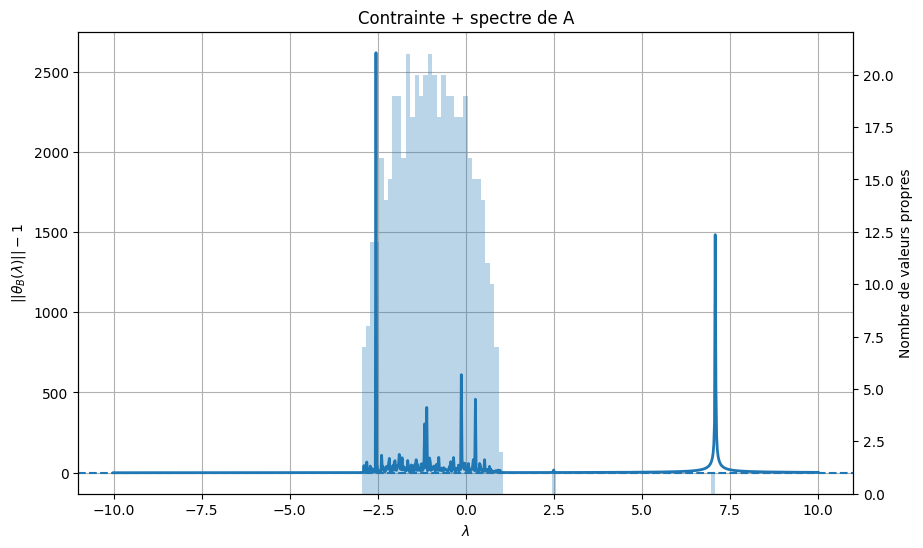
\includegraphics[width=\textwidth]{fig/lambda/contrainte.png}
        \caption{Full range.}
    \end{subfigure}
    \begin{subfigure}{0.32\textwidth}
        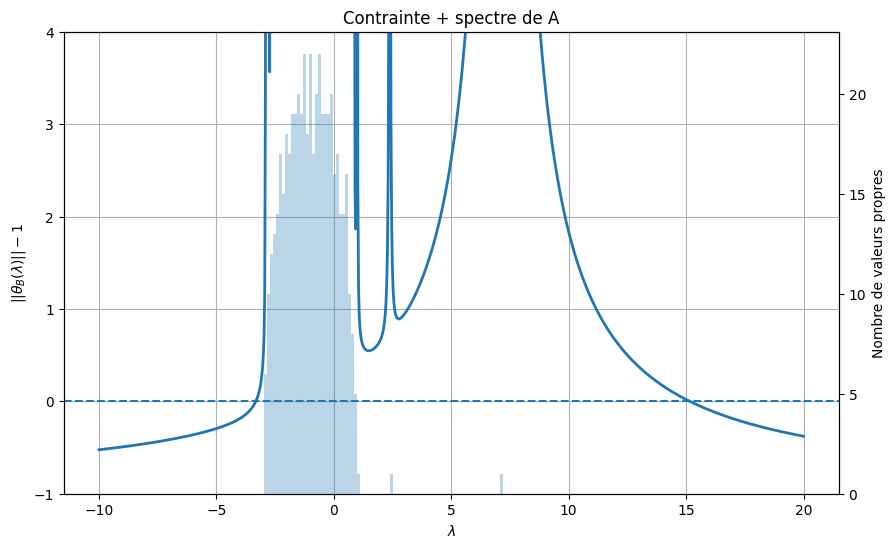
\includegraphics[width=\textwidth]{fig/lambda/contrainte_zoom.png}
        \caption{Zoom around the solution.}
    \end{subfigure}
    \begin{subfigure}{0.32\textwidth}
        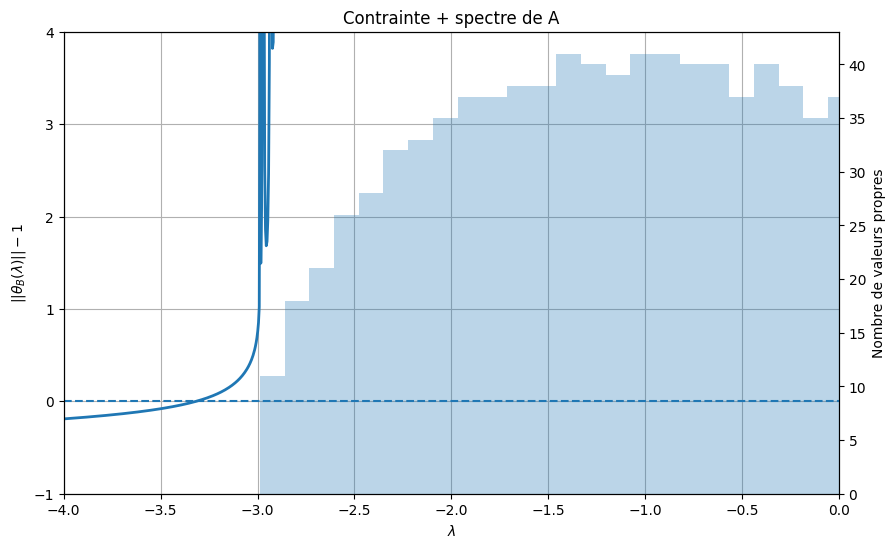
\includegraphics[width=\textwidth]{fig/lambda/contrainte_zoom_plus.png}
        \caption{Further zoom.}
    \end{subfigure}
    \caption{Norm of the estimator $\hat{\vect{x}}^{(2)}_B$ and spectrum of $\mathcal{H}_{\mathrm{EWC}}$ as a function of the Lagrange multiplier $\lambda$, for $n=1000$ and $\lambda_1=\lambda_2=3$. The norm equals $1$ at the unique root $\lambda^*$ of $g(\lambda)=0$ lying between two consecutive eigenvalues of $\vect{M}$.}
    \label{fig:Fisher_Hess}
\end{figure}



\subsection{Additional overlap figures}

\begin{figure}[H]
    \begin{subfigure}{0.45\textwidth}
        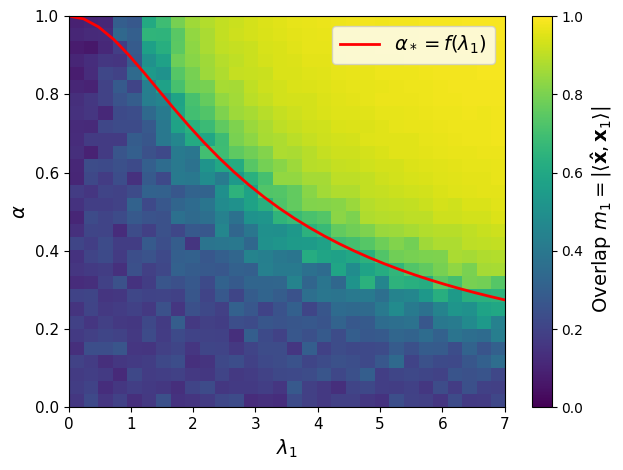
\includegraphics[width=\textwidth]{fig/m2spikes/alpha_vs_lambda1/m1_rho02.png}
                \caption{$\rho = 0.2$}
    \end{subfigure}
    \begin{subfigure}{0.45\textwidth}
    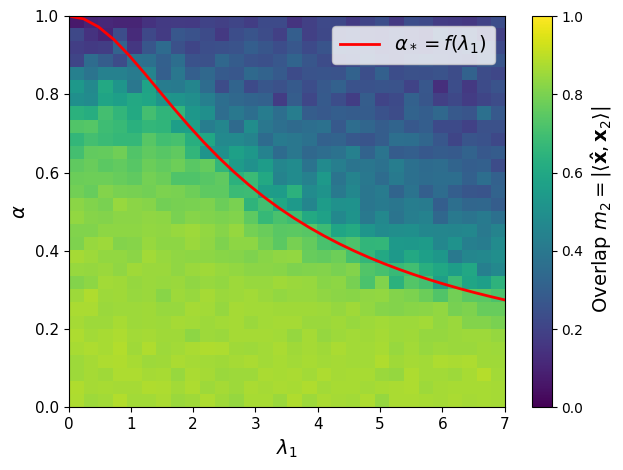
\includegraphics[width=\textwidth]{fig/m2spikes/alpha_vs_lambda1/m2_rho02.png}
            \caption{$\rho = 0.2$}
            \label{fig:m2_alpha_vs_lambda1}
    \end{subfigure}
    \begin{subfigure}{0.45\textwidth}
        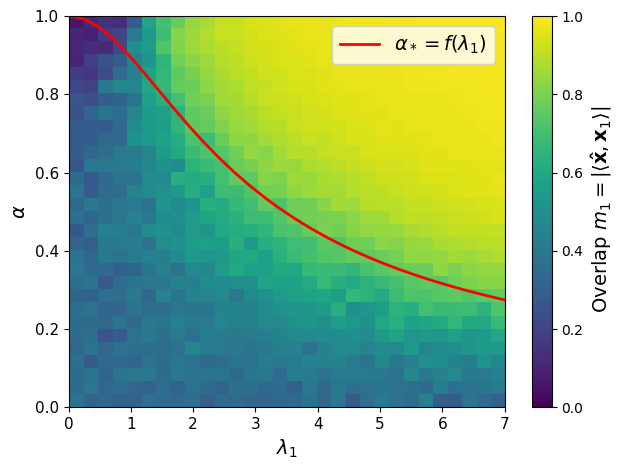
\includegraphics[width=\textwidth]{fig/m2spikes/alpha_vs_lambda1/m1_rho04.png}
                \caption{$\rho = 0.4$}
    \end{subfigure}
    \begin{subfigure}{0.45\textwidth}
    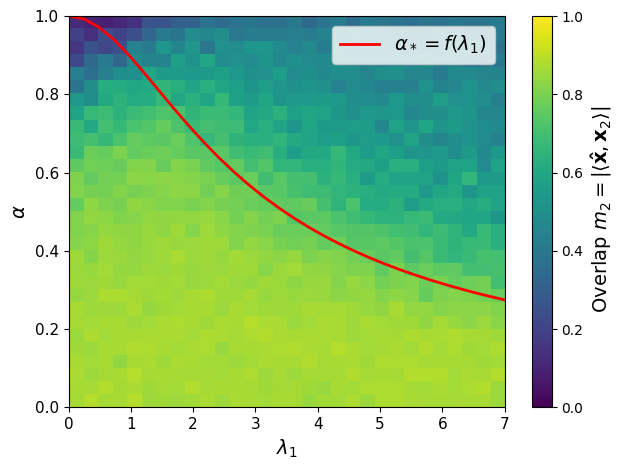
\includegraphics[width=\textwidth]{fig/m2spikes/alpha_vs_lambda1/m2_rho04.png}
            \caption{$\rho = 0.4$}
            \label{fig:m2_alpha_vs_lambda1}
    \end{subfigure}
    \begin{subfigure}{0.45\textwidth}
    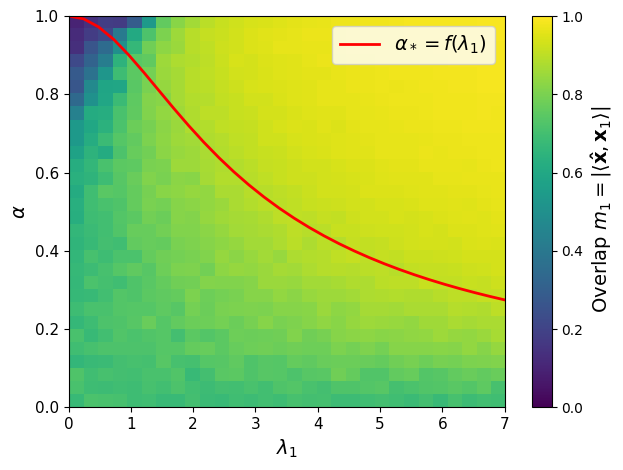
\includegraphics[width=\textwidth]{fig/m2spikes/alpha_vs_lambda1/m1_rho08.png}
                \caption{$\rho = 0.8$}
                \label{fig:m2_alpha_vs_lambda1}
    \end{subfigure}
    \hfill
    \begin{subfigure}{0.45\textwidth}
    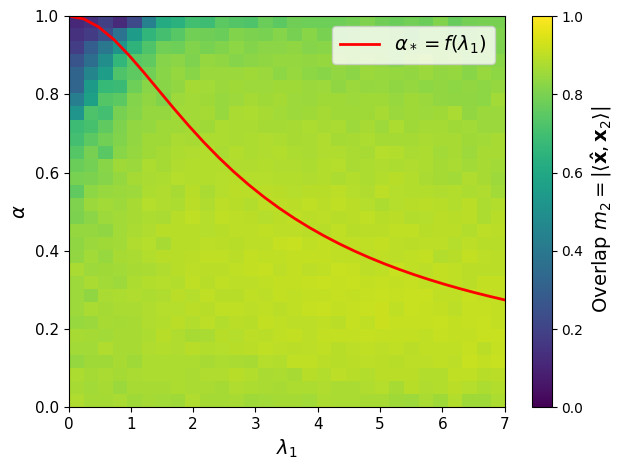
\includegraphics[width=\textwidth]{fig/m2spikes/alpha_vs_lambda1/m2_rho08.png}
            \caption{$\rho = 0.8$}
            \label{fig:m2_alpha_vs_lambda1}
    \end{subfigure}

   \caption{Overlaps $m$ as a function of the importance factor $\alpha$ and $\lambda_1$, for the first signal $\vect{x}_1$ (left column) and the second signal $\vect{x}_2$ (right column), for increasing values of $\rho \in \{0.2, 0.4, 0.8\}$. Fixed parameters: $\lambda_2=2$, $n=200$. Each overlap is averaged over 10 simulations. The red line shows $\alpha_*=f(\lambda_1)$ from Eq.~\eqref{eq:4.8}.}
    \label{fig:m_alpha_vs_lambda1}
\end{figure}




\paragraph{Limit  $k_i < 1$}

To analyse this limit:

ZOOM on the part where $\lambda_1 \in [0,1]$ for $\lambda_2 >1$, to see if we can have the info on $u_1$.


\begin{figure}[H] 
   \begin{subfigure}{0.5\textwidth}
        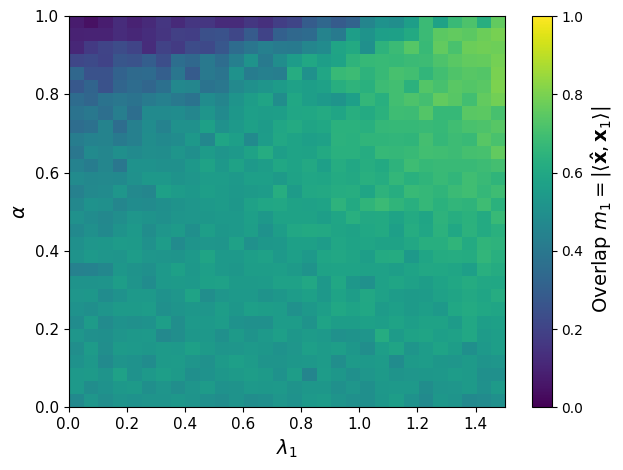
\includegraphics[width=\textwidth]{fig/m2spikes/limit/m1rho06.png}
                \caption{}
    \end{subfigure}
    \begin{subfigure}{0.5\textwidth}
    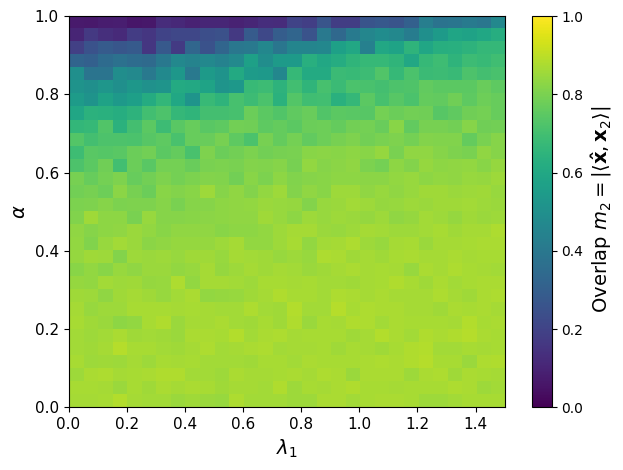
\includegraphics[width=\textwidth]{fig/m2spikes/limit/m2rho06.png}
            \caption{}
    \end{subfigure}
  \caption{\centering Overlaps $m$ as function of $\lambda_1$ and the importance factor $\alpha$ for (a) the first signal $x_1$, (b) the second $x_2$. With the fixed parameters:  $\lambda_2=2$ and a correlation $\rho =0.6$. The simulation is done for dimension of the spikes $n=200$ and the overlap is computed as the mean overlap over 10 simulations.}

\end{figure}
\begin{figure}[H] 
   \begin{subfigure}{0.5\textwidth}
        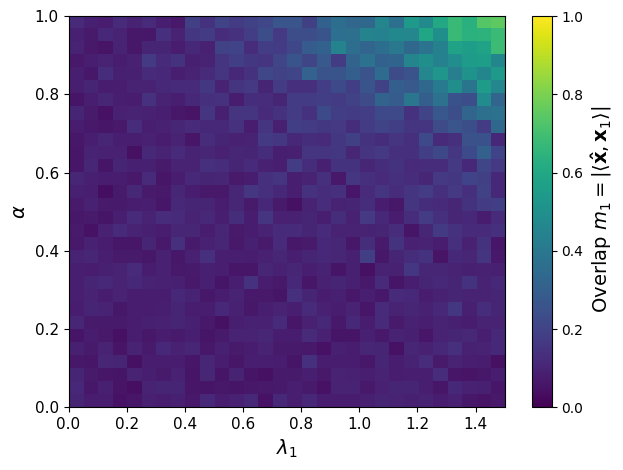
\includegraphics[width=\textwidth]{fig/m2spikes/limit/m1rho0.png}
                \caption{}
    \end{subfigure}
    \begin{subfigure}{0.5\textwidth}
    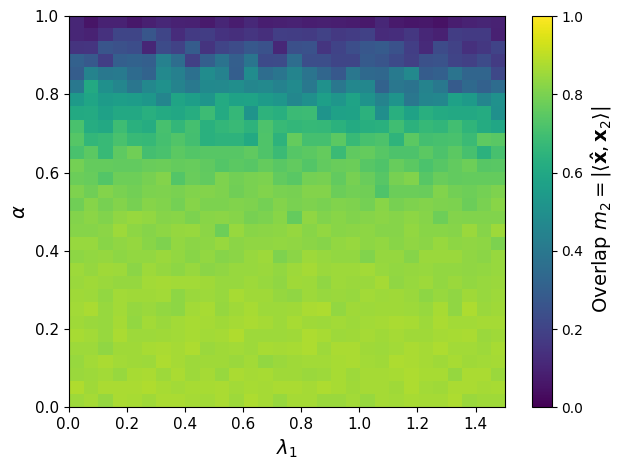
\includegraphics[width=\textwidth]{fig/m2spikes/limit/m2rho0.png}
            \caption{}
    \end{subfigure}
  \caption{\centering Overlaps $m$ as function of $\lambda_1$ and the importance factor $\alpha$ for (a) the first signal $x_1$, (b) the second $x_2$. With the fixed parameters:  $\lambda_2=2$ and a correlation $\rho =0$. The simulation is done for dimension of the spikes $n=200$ and the overlap is computed as the mean overlap over 10 simulations.}
  
\end{figure}

we 
\begin{figure}[H] 
   \begin{subfigure}{0.5\textwidth}
        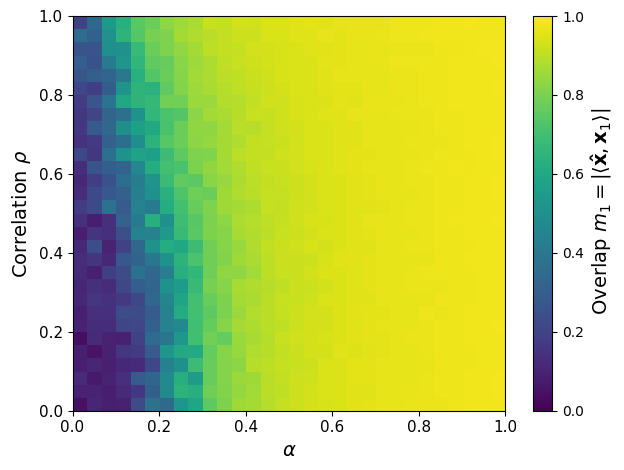
\includegraphics[width=\textwidth]{fig/m2spikes/limit/m1_rho_alpha_lambda20.8_l15.png}
                \caption{}
    \end{subfigure}
    \begin{subfigure}{0.5\textwidth}
    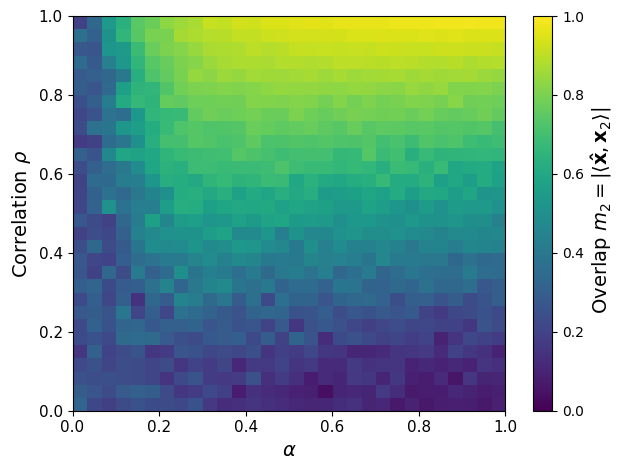
\includegraphics[width=\textwidth]{fig/m2spikes/limit/m2_rho_alpha_lambda20.8_l15.png}
            \caption{}
    \end{subfigure}
  \caption{\centering Overlaps $m$ as function of the correlation $\rho$ and the importance factor $\alpha$ for (a) the first signal $x_1$, (b) the second $x_2$. With the fixed parameters:  $\lambda_2=0.8$ and $\lambda_1 =5$. The simulation is done for dimension of the spikes $n=200$ and the overlap is computed as the mean overlap over 10 simulations.}

  
\end{figure}

\begin{figure}[H] 
   \begin{subfigure}{0.5\textwidth}
        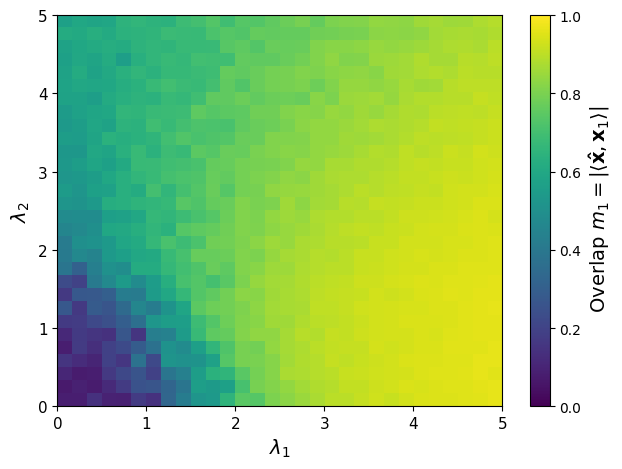
\includegraphics[width=\textwidth]{fig/m2spikes/limit/m1_lambda1_lambda_2_rho06_alpha05.png}
                \caption{}
    \end{subfigure}
    \begin{subfigure}{0.5\textwidth}
    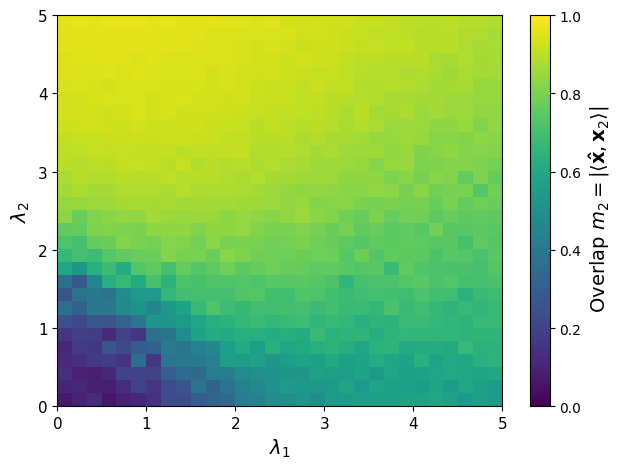
\includegraphics[width=\textwidth]{fig/m2spikes/limit/m2_lambda1_lambda_2_rho06_alpha05.png}
            \caption{}
    \end{subfigure}
  \caption{\centering Overlaps $m$ as function  $\lambda_1$ and $\lambda_2$ for (a) the first signal $x_1$, (b) the second $x_2$. With the fixed parameters:  $\rho=0.6$ and $\alpha = \sqrt{1/2}$ . The simulation is done for dimension of the spikes $n=200$ and the overlap is computed as the mean overlap over 10 simulations.}
\end{figure}



\paragraph{Proof of Prop. \ref{proof_tali_1}}
\begin{proof}
Let $W$ be a symmetric random matrix with $\mathbb{E}[W_{ij}] = 0$ and
\[
\mathbb{E}[W_{ij} W_{k\ell}] = \sigma^2 (\delta_{ik}\delta_{j\ell} + \delta_{i\ell}\delta_{jk}).
\]
For a fixed matrix $\vect A$, one can compute entry-wise:
\[
(W A W)_{ij} = \sum_{k,\ell} W_{ik} A_{k\ell} W_{\ell j}
\]
Taking expectation and using the covariance above,
\[
\mathbb{E}[(\vect W \vect A \vect W)_{ij}]
= \sigma^2 \sum_{k,\ell} A_{k\ell} (\delta_{i\ell}\delta_{kj} + \delta_{ij}\delta_{k\ell})
= \sigma^2 (A_{ji} + \delta_{ij}\mathrm{Tr}(\vect A)).
\]
Hence
\[
    \mathbb{E}[\vect W \vect A \vect W] = \sigma^2(\mathrm{Tr}(\vect A) \vect I + \vect A^\top)
\]
\end{proof}


\end{document}
